\documentclass[12pt,a4paper,twoside]{stb}

\usepackage{cmap}
\usepackage[T2A]{fontenc}
\usepackage[utf8x,utf8]{inputenc}
\usepackage[english,russian]{babel}
\usepackage{ucs} 
\usepackage{textcase}

\pdfpkresolution=2400
\pdfpkmode={supre}

\usepackage{amsmath,amssymb,amsthm,xspace,ifthen,graphicx}

\usepackage[
  pdftitle={Security Requirements for Software Cryptographic Modules},
  pdfauthor={},
  bookmarks=true,
  pdfpagemode=UseOutlines,
  pdfstartview=FitH,
  linkcolor=black,
  citecolor=black]{hyperref}

\usepackage[usenames,dvipsnames]{color}
\usepackage{listings}

\usepackage{ulem}
\normalem

\usepackage{longtable}
\setlongtables

\usepackage{defs}

\renewcommand{\baselinestretch}{1.1}
\renewcommand{\thefootnote}{}
\setcounter{tocdepth}{1}
\pagestyle{headings}

\hoffset          = -1in 
\voffset          = -1in
\oddsidemargin    = 30mm             % стандарт ТКП 1.5-2004            
\evensidemargin   = 10mm             % верхнее = 20 мм                  
\textwidth        = 170mm            % правое  = 10 мм                  
\topmargin        = 20mm             % левое и нижнее = не менее 20 мм  
\textheight       = 252mm  
\headsep          = 1\baselineskip
\headheight       = 2\baselineskip
\addtolength{\topmargin}{-\headheight}
\addtolength{\topmargin}{-\headsep}
\parindent        = 0.8cm

\begin{document}
\begin{sloppypar}
\renewcommand\figurename{Рисунок}
\renewcommand\tablename{Таблица}
\renewcommand\contentsname{Содержание}
\renewcommand\bibname{Библиография}

\def\draftlogo{\scshape\small СТБ 34.101.27-2011}

\pagestyle{myheadings}

\thispagestyle{empty}

\noindent
\begin{tabular}{lcr}
{\bf ГОСУДАРСТВЕННЫЙ СТАНДАРТ}  & \hspace{3.5cm}   & 
{\bf \draftlogo}\\
{\bf РЕСПУБЛИКИ~БЕЛАРУСЬ} & \\
\end{tabular}

\hrule height 1pt
\vskip0.4mm
\hrule height 2pt

\vskip2cm
\noindent
{\bf\Large Информационные технологии и безопасность}\\[10pt]
{\bf\large ТРЕБОВАНИЯ БЕЗОПАСНОСТИ К ПРОГРАММНЫМ}\\
{\bf\large СРЕДСТВАМ КРИПТОГРАФИЧЕСКОЙ ЗАЩИТЫ}\\
{\bf\large ИНФОРМАЦИИ}

\vskip2cm
\noindent
{\bf\Large Iнфармацыйныя тэхналогii i бяспека}\\[10pt]
{\bf\large ПАТРАБАВАННI БЯСПЕКI ДА ПРАГРАМНЫХ СРОДКАЎ}\\
{\bf\large КРЫПТАГРАФIЧНАЙ АХОВЫ IНФАРМАЦЫI}

\noindent
%{\em Настоящий проект предстандарта не подлежит применению до его утверждения}

\vskip12cm
\hrule height 1pt
\vskip0.4mm
\hrule height 2pt
\noindent
\begin{tabular}{p{5cm}cp{4cm}}
\vtop{\null\hbox{{
\includegraphics[width=2.6cm]{figs/stb}}}} & \hspace{6cm} & 
\mbox{}\newline\mbox{}\newline\newline Госстандарт\newline Минск\\
\end{tabular}

\pagebreak


\hrule
\vskip2mm

УДК~004.4.056.55(083.74)(476)\hfill
МКС~35.240.40\hfill
КП~05

\vskip0.5mm

{\bf Ключевые слова}: технологии информационные, безопасность,
криптографическая защита информации, 
программное средство криптографической защиты информации 

\vskip0.5mm

\hrule 

\rule{0pt}{5mm}
	 
\centerline{\bf Предисловие} 

Цели, основные принципы, положения по государственному регулированию и 
управлению в области технического нормирования и стандартизации 
установлены Законом Республики Беларусь <<О техническом нормировании и 
стандартизации>>.  

\vskip0.2cm

1~РАЗРАБОТАН учреждением Белорусского государственного университета
<<Науч\-но-исследовательский институт прикладных проблем математики и информатики>>

ВНЕСЕН Оперативно-аналитическим центром при Президенте Республики Беларусь (ОАЦ)

2~УТВЕРЖДЕН и ВВЕДЕН В ДЕЙСТВИЕ постановлением Госстандарта Республики 
Беларусь от 25 ноября 2011 г. \No~83 

3~ВЗАМЕН СТБ П 34.101.27-2007 

\vfill

\hrule
\vskip1mm
Издан на русском языке

\pagebreak

\setcounter{page}{3}
\tableofcontents
\newpage
\mbox{}
\thispagestyle{empty}
\newpage
\setcounter{page}{3}

\pagestyle{headings}

\newpage
\setcounter{page}{1}
\pagestyle{headings}

\begin{center}
{\bfseries
ГОСУДАРСТВЕННЫЙ СТАНДАРТ РЕСПУБЛИКИ~БЕЛАРУСЬ
%\footnote{Версия 2.6}
\vskip 2pt
\hrule width\textwidth

\vskip 9pt

Информационные технологии и безопасность

ТРЕБОВАНИЯ БЕЗОПАСНОСТИ К ПРОГРАММНЫМ СРЕДСТВАМ КРИПТОГРАФИЧЕСКОЙ 
ЗАЩИТЫ ИНФОРМАЦИИ

\vskip 9pt

Iнформацыйныя тэхналогii i бяспека

ПАТРАБАВАННI БЯСПЕКI ДА
ПРАГРАМНЫХ СРОДКАЎ КРЫПТАГРАФIЧНАЙ АХОВЫ IНФАРМАЦЫI
}
% bfseries

\vskip 9pt

Information technologies and security

Security requirements for software cryptographic modules

\vskip 4pt                
\hrule width \textwidth
\end{center}

\mbox{}\hfill{\bfseries Дата введения 2012-03-01}



\chapter{Область применения}\label{Scope}

Настоящий государственный стандарт устанавливает 
общие требования безопасности к программным средствам,
которые используются для криптографической защиты информации
ограниченного распространения (за исключением государственных секретов). 

Стандарт предназначен для использования:
\begin{itemize}
\item[--]
заказчиками (потребителями) при задании требований безопасности к
программным средствам криптографической защиты информации;

\item[--]
разработчиками при создании 
программных средств криптографической защиты информации;

\item[--]
экспертами при оценке надежности
программных средств криптографической защиты информации.
\end{itemize}


%\chapter{Нормативные ссылки}\label{Refs}

В настоящем cтандарте использованы ссылки на следующие 
технические нормативные правовые акты в области 
технического нормирования и стандартизации (далее~--- ТНПА):

%\doubt{СТБ 34.101.31-2010 Информационные технологии и безопасность. 
%Криптографические алгоритмы шифрования и контроля целостности}

%\doubt{ГОСТ 28147-89 Системы обработки информации. 
%Защита криптографическая. Алгоритм криптографического преобразования}

\begin{remark}
При пользовании настоящим стандартом целесообразно 
проверить действие ТНПА по каталогу,
составленному на 1 января текущего года, и по соответствующим 
информационным указателям, опубликованным в текущем году.

Если ссылочные ТНПА заменены (изменены), то при пользовании настоящим 
стандартом следует руководствоваться замененными (измененными) ТНПА. 
Если ссылочные ТНПА отменены без замены, то положение, в котором 
дана ссылка на них, применяется в части, не затрагивающей эту ссылку.
\end{remark}



\chapter{Термины и определения}\label{Terms}

В настоящем стандарте применяют  
%
%термины в соответствии с СТБ 1176.1-99, СТБ 1176.2-99,
%СТБ~34.101.1~--- СТБ~34.101.3, 
%СТБ 1221, СТБ~34.101.31, ГОСТ 28147-89,
%а также 
%
следующие термины с соответствующими определениями:

{\bf \thedefctr~аутентификация:}
Проверка подлинности идентификатора оператора.

%Authenticate: To confirm the identity of an entity when that identity is presented.

{\bf \thedefctr~аутентификационные данные:}
Информация, которая используется для аутентификации.

%Information used to verify the claimed identity of a user

{\bf \thedefctr~генератор случайных чисел:}
Аппаратно-программное устройство, 
которое вырабатывает последовательность непредсказуемых 
элементов.

%aппаратно-программное устройство, 
%вырабатывающее последовательность чисел, 
%каждый следующий элемент которой трудно
%предсказать по всем предыдущим элементам.

{\bf \thedefctr~долговременный объект:}
Объект, который хранится в пределах криптографической границы или передается
за ее пределы, операции над которым могут выполняться в нескольких сеансах.

{\bf \thedefctr~зашифрование}:
Преобразование объектов,
направленное на обеспечение их конфиденциальности,
которое осуществляется с использованием секретного или открытого ключа.

% belt: Преобразование сообщения,
% направленное на обеспечение его конфиденциальности,
% которое определяется с использованием ключа.

{\bf \thedefctr~защита объектов:}
Контроль целостности и обеспечение конфиденциальности критических объектов,
контроль целостности открытых объектов.

{\bf \thedefctr~идентификация:}
Присвоение операторам уникальных идентификаторов.

{\bf \thedefctr~имитовставка}:
Контрольная характеристика объекта, 
которая определяется с использованием секретного ключа 
и служит для контроля целостности и подлинности объекта.

% belt: Двоичное слово, 
% которое определяется по сообщению с использованием ключа 
% и служит для контроля целостности и подлинности сообщения.

{\bf \thedefctr~имитозащита}:
Контроль целостности объектов, 
который реализуется путем выработки и проверки имитовставок.

% old: Выработка или проверка имитовставок.

% belt, brng: Контроль целостности сообщений, 
% который реализуется путем выработки и проверки имитовставок.

{\bf \thedefctr~клиентская программа:}
Программа, которая от лица оператора вызывает сервисы
программного средства криптографической защиты информации.

{\bf \thedefctr~конфиденциальность}:
Гарантия того, что объекты доступны для использования
только тем сторонам, которым они предназначены.

{\bf \thedefctr~криптографическая граница:} 
Точно определенный разработчиком непрерывный физический 
периметр в среде эксплуатации, 
который определяет контролируемую границу программного средства 
криптографической защиты информации.

{\bf \thedefctr~криптографический алгоритм:}
Алгоритм преобразования объектов,
направленный на обеспечение их конфиденциальности,
контроля целостности или подлинности,
в том числе алгоритм управления криптографическими
ключами для защиты объектов.

{\bf \thedefctr~криптографический ключ:} 
Объект-параметр, используемый вместе с криптографическим алгоритмом 
для управления операциями зашифрования и расшифрования,
вычисления и проверки электронной цифровой подписи,
выработки и проверки имитовставки,
выработки псевдослучайных данных,
выработки совместно используемой конфиденциальной информации.

% bign: Параметр, который управляет криптографическими 
% операциями зашифрования и расшифрования, 
% выработки и проверки ЭЦП, 
% генерации псевдослучайных чисел и др.

{\bf \thedefctr~криптографический протокол:}
Точно определенные последовательность действий или набор правил, 
предусматривающие взаимодействие двух и более сторон 
с использованием криптографических алгоритмов.

{\bf \thedefctr~критические системные компоненты:}
Находящееся внутри криптографической границы 
аппаратное и программное обеспечение, которое используется
для передачи, обработки и хранения объектов
программного средства криптографической защиты информации.

{\bf \thedefctr~критический объект:} 
Объект, несанкционированные раскрытие или модификация которого 
снижают безопасность.

{\bf \thedefctr~личный ключ:}
Криптографический ключ, используемый
вместе с криптографическим алгоритмом с открытым ключом, 
который однозначно связан с конкретным оператором 
и не является общедоступным.

% bign: Ключ, который связан с конкретной стороной, не является общедоступным
% и используется в настоящем предстандарте для выработки ЭЦП 
% и для разбора токена ключа.

{\bf \thedefctr~неявная копия:}
Копия объекта, переданная по побочному каналу.

{\bf \thedefctr~объект}: 
Элемент, который содержит или получает информацию
и над которым выполняются операции.

{\bf \thedefctr~оператор:}
Лицо или клиентская программа, выступающая от имени лица, 
которые взаимодействуют с программным средством криптографической защиты 
информации.

{\bf \thedefctr~открытый объект:} 
Объект, несанкционированная модификация 
которого снижает безопасность, 
а раскрытие~--- не снижает.

{\bf \thedefctr~открытый ключ:}
Криптографический ключ, используемый 
вместе с криптографическим алгоритмом с открытым ключом, 
который строится по личному ключу  
и может быть сделан общедоступным.

% bign: Ключ, который строится по личному ключу, 
% связан с конкретной стороной, 
% может быть сделан общедоступным
% и используется в настоящем предстандарте для проверки ЭЦП 
% и для создания токена ключа.

{\bf \thedefctr~побочный канал}:
Нежелательный дополнительный канал передачи информации о 
входных, промежуточных или выходных данных 
криптографического алгоритма или протокола, 
возникающий из-за особенностей его 
аппаратно-программной реализации.

{\bf \thedefctr~подлинность}:
Гарантия того, что сторона действительно 
является владельцем (создателем, отправителем) 
определенного объекта.

{\bf \thedefctr~политика управления доступом}:
Правила, определяющие допустимые операции 
операторов над сервисами и объектами.

{\bf \thedefctr~программное средство криптографической защиты информации;
\TOE}:
Средство криптографической защиты информации, выполненное целиком 
программно, без аппаратных компонентов.

{\bf \thedefctr~разделение секрета}:
Разбиение критического объекта на частичные секреты, 
каждый из которых по отдельности или даже вместе с некоторыми
другими частичными секретами не дает информации об исходном объекте.

{\bf \thedefctr~расшифрование}:
Преобразование, обратное зашифрованию, которое определяется с помощью
секретного или личного ключа.

% belt: Преобразование, обратное зашифрованию.

{\bf \thedefctr~сеанс оператора:}
Период взаимодействия оператора с программным средством криптографической
защиты информации.

{\bf \thedefctr~сеансовый объект:}
Объект, который создается, 
используется и уничтожается в течение одного сеанса.

{\bf \thedefctr~секрет аутентификации:}
Пароль, PIN-код и другие аутентификационные данные, 
которые однозначно связаны с конкретным оператором 
и не являются общедоступными.

{\bf \thedefctr~секретный ключ:}
Криптографический ключ, используемый
вместе с криптографическим алгоритмом с секретным ключом, 
который однозначно связан с конкретным оператором 
или группой операторов и не является общедоступным.

% belt: Параметр, который управляет операциями шифрования 
% и имитозащиты и который известен только определенным сторонам.

{\bf \thedefctr~сервис:}
Реализованная в программном средстве криптографической защиты информации 
и доступная оператору функция.

{\bf \thedefctr~синхропосылка:}
Открытые входные данные криптографического алгоритма или протокола,
которые обеспечивают уникальность результатов 
криптографического преобразования на фиксированном ключе.

% belt: Открытые входные данные криптографического алгоритма,
% которые обеспечивают уникальность результатов 
% криптографического преобразования на фиксированном ключе.

{\bf \thedefctr~системный сеанс:}
Непрерывный период работы программного средства криптографической 
защиты информации.

{\bf \thedefctr~среда экcплуатации}:
Аппаратно-программное обеспечение, 
организационные процедуры и мероприятия, 
необходимые для функционирования 
программного средства криптографической защиты информации.

{\bf \thedefctr~средство криптографической защиты информации;
СКЗИ}:
Набор аппа\-ратно-программных компонентов, 
который реализует криптографические алгоритмы и протоколы,
а также возможно дополнительные средства управления ключами,
контроля доступа и проверки работоспособности, 
предназначенные для безопасного управления вызовами
криптографических алгоритмов и их входными и выходными данными.

{\bf \thedefctr~целостность}:
Гарантия того, что объект не изменен при хранении или передаче.

{\bf \thedefctr~шифрование}:
Зашифрование или расшифрование.

{\bf \thedefctr~хэш-значение}:
Контрольная характеристика объекта, 
которая определяется без использования ключа и 
служит для контроля целостности объекта и для представления 
объекта в сжатой форме.

% belt, bign: Двоичное слово фиксированной длины, 
% которое определяется по сообщению без использования ключа и 
% служит для контроля целостности сообщения и для представления 
% сообщения в сжатой форме.

{\bf \thedefctr~хэширование}:
Выработка хэш-значений.

% belt: +

{\bf \thedefctr~частичный секрет}:
Критический объект, 
полученный в результате применения метода разделения секрета.

% bels: конфиденциальные данные пользователя, используемые для 
% восстановления секрета

{\bf \thedefctr~электронная цифровая подпись; ЭЦП}:
Контрольная характеристика объекта, 
которая определяется с использованием личного ключа, 
проверяется с использованием открытого ключа,
служит для контроля целостности и подлинности объекта 
и обеспечивает невозможность отказа от авторства.

% bign: Двоичное слово, которое служит для контроля 
% целостности и подлинности сообщения, 
% обеспечивает невозможность отказа от авторства,
% определяется с использованием личного ключа и проверяется 
% с использованием открытого ключа.




\chapter{Оформление требований безопасности}\label{Notations}

Требования безопасности разбиваются на группы.
Группы обозначаются двухбуквенными кодами:
КП, РС, УД и др.
%
Требования внутри группы нумеруются последовательно, 
начиная с~единицы.

Требования безопасности задают разбиение~\TOE на два класса.
%
Для каждого требования в круглых скобках перечисляются 
классы~\TOE, на которые требования распространяются.
Возможные варианты: (1), (2) или (1, 2).

В тексте имеются ссылки на требования. Ссылка [T] означает,
что условия требования~T должны быть использованы в месте ссылки.
Ссылка \{T\} означает, что условия или пояснения в месте ссылки
детализируют~T. 

Формулировки требований безопасности могут включать указания на 
необходимость определения списка методов, списка компонентов, 
списка средств и др.
%
Если не оговорено противное, то результатом определения 
может быть пустой список.

\providecommand{\CryptoDisk}{<<{Криптодиск}>>\xspace}

\chapter{Общие положения}\label{Common}

\section{Назначение}

Настоящий стандарт устанавливает требования безопасности к программным 
средствам криптографической защиты информации.
ПСКЗИ представляет собой набор программ и связанных с ними данных,
который реализует криптографические алгоритмы и протоколы,
а также дополнительно:
\begin{itemize}
\item[--]
функции управления данными,
включая средства генерации, экспорта, импорта и уничтожения
ключей;

\item[--]
механизмы контроля доступа к данным,
включая средства идентификации и аутентификации;

\item[--]
механизмы проверки работоспособности,
включая средства тестирования, диагностики и 
контроля целостности,
%
предназначенные для безопасного управления вызовами
криптографических алгоритмов и их входными и выходными данными.
\end{itemize}

Требования безопасности делятся на 
функциональные~(разделы~\ref{FReqsTOE}, \ref{FReqsEnv}) 
и гарантийные~(раздел~\ref{AReqs}).
Функциональные требования направлены на решение задач безопасности,
гарантийные требования поддерживают качество решения данных задач.
%
Функциональные требования обеспечивают противодействие угрозам безопасности, 
следование определенным правилам безопасности.
%
Гарантийные требования обеспечивают доверие к тому, 
что программное средство корректно спроектировано и разработано, 
протестировано в достаточном объеме, 
правильно установлено и эксплуатируется.

Программы~\TOE выполняются в определенной среде эксплуатации~---
на персональном компьютере, в мобильном устройстве, на смарт-карте и др.
Среда эксплуатации обеспечивает~\TOE процессорными ресурсами, 
ресурсами памяти, а также предоставляет системные средства 
управления этими ресурсами.
%
Программное средство зависимо от ресурсов среды 
и не в состоянии обеспечить безопасность своих объектов самостоятельно.
Поэтому функциональные требования реализуются
как средствами~\TOE~(раздел~\ref{FReqsTOE}),
так и средствами среды~(раздел~\ref{FReqsEnv}).

Требования безопасности задают разбиение~\TOE
на два класса. К средствам первого класса выдвигается 
базовый набор требований, к средствам второго~--- усиленный.
%
Средства второго класса рекомендуется использовать
в тех случаях, когда возможны изменения критических системных 
компонентов в среде эксплуатации,
например, если разрешена установка новых программ,
обновление операционной системы, 
замена оборудования и др.
%
Средства второго класса рекомендуется применять также тогда,
когда гипотетический нарушитель имеет возможность 
наблюдать за побочными каналами,
например за временем выработки ЭЦП на смарт-карте.
	
Методы реализации требований безопасности 
описываются в функциональной спецификации. 
%
Функциональная спецификация может представлять собой 
отдельный документ либо разделы нескольких документов.
%
Примерное содержание функциональной спецификации представлено 
в приложении~\ref{SPEC}.
%
Приложение~\ref{EXAMPLE} содержит примерную спецификацию гипотетического 
программного средства~\CryptoDisk.

\section{Криптографическая поддержка}

\TOE реализует один или несколько криптографических алгоритмов 
или протоколов. Алгоритмы и протоколы используются 
как в доступных извне сервисах, 
так и во внутренних средствах безопасности, 
обеспечивающих защиту объектов.

Входные данные криптографического алгоритма делятся на служебные и собственно 
обрабатываемые (содержательные) объекты. 
К служебным объектам относятся долговременные параметры, 
которые задают семейство криптографических преобразований для данного алгоритма,
ключи, которые определяют выбор одного преобразования из семейства, 
синхропосылки, которые обеспечивают уникальность результатов 
преобразования на фиксированном ключе, и др.

Криптографические алгоритмы делятся на
алгоритмы с секретным ключом (симметричные),
алгоритмы с открытым ключом (асимметричные) 
и бесключевые алгоритмы.
%
В симметричных алгоритмах для выполнения нескольких связанных
операций, например зашифрования и расшифрования,
используется один и тот же секретный ключ. 
%
В асимметричных алгоритмах используется пара ключей~--- 
личный и соответствующий ему открытый.
Например, в алгоритмах ЭЦП при выработке подписи используется 
личный ключ, а при ее проверке~--- открытый.
%
К бесключевым относятся алгоритмы хэширования, 
алгоритмы разделения секрета, 
алгоритмы построения семейства ключей по одному главному ключу. 
В этих алгоритмах ключи, отвечающие за выбор 
криптографического преобразования,
не используются, хотя обрабатываемые объекты сами могут являться 
ключами~\forref{CryptoAlg}.

При реализации криптографических алгоритмов разрешается 
сужать множество обрабатываемых объектов. 
Например, алгоритм шифрования может обрабатывать сообщения не любой,
а только определенной длины.
Вместе с тем сужение множества ключей не допускается~\forref{CryptoAlg}.

Кроме собственно криптографических алгоритмов, их спецификации могут 
определять методы генерации долговременных параметров и ключей.
Методы могут определяться рамочно, без исчерпывающих деталей.
%
Например, при генерации параметров ЭЦП на основе эллиптических кривых 
используются вспомогательные алгоритмы проверки простоты чисел, 
расчета порядка группы точек эллиптической кривой, 
извлечения квадратных корней и др., 
которые могут быть не определены в спецификации.
%
При реализации в~\TOE методов генерации параметров проводится 
уточнение вспомогательных алгоритмов.
%
Уточнения могут касаться также способов генерации случайных чисел,
по которым строятся искомые долговременные параметры или ключи~\forref{CryptoGen}.

Криптографические протоколы представляют собой наборы 
криптографических алгоритмов, которые выполняются в определенной
последовательности двумя (или более) сторонами. 
Для протоколов также справедливы приведенные выше пояснения.

В~\TOE реализуются средства тестирования криптографических алгоритмов 
и протоколов. Для тестирования могут использоваться:
тесты известного ответа, тесты прямого и обратного преобразований, 
тесты на соответствие между открытым и личным ключами~\forref{SelfTests}.

\section{Операторы}

С~\TOE взаимодействуют операторы.
%
Взаимодействие состоит в работе с сервисами.
%
При использовании сервиса оператор 
готовит и передает входные данные и управляющие параметры сервиса,
вызывает сервис, получает и обрабатывает выходные данные.

Некоторые операции могут выполняться не одним, а несколькими сервисами. 
Например, защита канала связи может быть реализована сервисом 
выработки общего сеансового ключа и сервисом шифрования данных канала.
Определенные последовательности вызовов сервисов могут быть запрещены. 
Например, запрещено выполнять шифрование до выработки 
общего сеансового ключа~\forref{Services}.

Сервисы доступны операторам через устройства ввода/вывода 
(клавиатуру, дисплей, принтер, порты) и логические интерфейсы
(например, наборы функций динамических библиотек).
%
Оператор может взаимодействовать с~\TOE не напрямую, 
а через клиентские программы (клиентов электронной почты, браузеры, 
программы управления электронными документами). 
%Клиентские программы выступают от лица операторов и отождествляются с ними.

\TOE поддерживает определенные роли (категории) операторов.
Имеется роль <<Администраторы>>.
Операторы этой роли наделены правами выполнять 
административные сервисы~\TOE:
устанавливать и настраивать~\TOE, 
управлять правами операторов, вводить мастер-ключи.
%
Рекомендуется определять роль <<Пользователи>>.
Пользователи выполняют общие сервисы \TOE:
шифруют почтовые отправления, проверяют ЭЦП электронных документов,
генерируют ключи~\forref{DAC}.

Имеется предопределенная роль <<Система>>,
которая явно может не определяться.
Неявный оператор этой роли (системный оператор)
выполняет внутренние сервисы~\TOE:
самотестирование при загрузке, 
контроль доступа, управление состояниями сеансов.

%Могут вводиться дополнительные роли.
Один и тот же оператор может выполнять сразу несколько 
ролей~\forref{Identification}.

\section{Аутентификация}

В~среде эксплуатации~\TOE реализуются средства аутентификации 
для проверки принадлежности оператора к явным ролям 
и допустимости выполнения оператором 
сервисов данных ролей. 
%
Аутентификация требуется также для проверки прав доступа вызываемых 
оператором сервисов к открытым и критическим объектам. 
Полный доступ к таким объектам разрешается, как правило,
только владельцам и для проверки полномочности доступа кроме 
роли, используется также идентификатор оператора.
%
Допускается, что для выполнения некоторых сервисов 
или доступа к некоторым 
объектам требуется дополнительная аутентификация~\forref{Authentication}.

Средства аутентификации могут быть полностью или частично реализованы 
самим~\TOE.

Методы аутентификации
основываются на использовании комбинаций из трех факторов: 
владение операторами устройствами аутентификации (<<что я имею>>), 
знание секретов аутентификации (<<что я знаю>>), 
обладание биометрическими характеристиками (<<кто я>>).
Рекомендуется задействовать более одного фактора, например использовать 
карты доступа вместе с PIN-кодами доступа~\forref{Auth2Factor}.

При аутентификации операторы предъявляют
устройства аутентификации (смарт-карты) 
и вводят аутентификационные данные (пароли, отпечатки пальцев).
%
Средства аутентификации проверяют корректность представленных устройств и 
сравнивают характеристики аутентификационных данных 
с контрольными значениями.

При создании и изменении секретов аутентификации предусматривается 
проверка их качества. Проверка может состоять в контроле 
длины пароля или контроле включения в пароль как цифровых, 
так и буквенных символов в различных регистрах.
Проверка качества секретов не может основываться на ограничениях 
в руководствах, \ie на предположении о том, что оператор
обязательно задаст пароль нужного качества~\forref{PwdSet}.

\section{Сеансы}

Взаимодействие оператора с~\TOE происходит в форме сеансов. 
В начале сеанса, как правило, 
выполняются сервисы идентификации и аутентификации оператора,
в конце сеанса~--- очистка и уничтожение сеансовых объектов.
%
Отдельно выделяется системный сеанс неявного системного оператора,
который совпадает с непрерывным периодом работы~\TOE
(от загрузки до выгрузки программ). 

Системный сеанс~\TOE может находиться в одном из нескольких состояний,
которые характеризуются различными правами доступа к сервисам. 
%
Имеются состояния, соответствующие сеансам операторов различных ролей. 
В этих состояниях операторы могут выполнять сервисы в соответствии 
с политикой управления доступом. 
%
Имеется также состояние блокировки,
в котором выполнение сервисов запрещается или сильно ограничивается.
%
Примеры других состояний системного сеанса:
<<самотестирование>>,
<<ожидание>> (до аутентификации операторов),
<<временная блокировка>> (блокировка на определенный период времени
после превышения порога неудачных попыток аутентификации) и др.
%
Могут определяться подчиненные состояния,
например внутренние состояния сеансов администратора и пользователя~\forref{States}.

Блокировка может состоять в принудительном завершении программ~\forref{LockState}.

Многозадачные операционные системы могут поддерживать 
одновременное выполнение сеансов для нескольких операторов~\TOE.
При этом состояния <<сеанс администратора>>, 
<<сеанс пользователя>> могут дублироваться. 
Считается, что~\TOE одновременно может находиться
сразу во всех состояниях, соответствующих сеансам операторов. 
Такой режим реализуется средствами обеспечения 
многозадачности операционной системы~\forref{States}.

%Один из возможных способов организации такой 
%поддержки состоит в следующем (рисунок~\ref{Fig.Descr.Session}).
%Клиентская программа является отдельным процессом операционной системы 
%с~защищенным от других процессов адресным пространством.
%Сеансами являются отдельные потоки клиентского процесса. 
%Данные сеансов одного процесса не защищены друг от друга,
%но защищены от данных сеансов других процессов.
%Для одновременного доступа к одним и тем же объектам
%нескольких сеансов средствами~\TOE или операционной системы 
%реализуются механизмы синхронизации.

\section{Объекты}

С помощью сервисов операторы выполняют операции над объектами~---
ключами, открытыми текстами, параметрами криптографических алгоритмов,
сертификатами открытых ключей и др.

Объекты делятся на открытые (общедоступные) 
и критические (ограниченного доступа).
%
Например, открытый ключ подписи является открытым объектом,
личный ключ подписи~--- критическим~\forref{Objects}.

Кроме этого, объекты делятся на сеансовые и долговременные.
Сеансовые объекты создаются во время сеансов операторов и уничтожаются
при их завершении. 
Доступ к таким объектам имеет только оператор сеанса.
Долговременные объекты существуют как во время, 
так и вне времени выполнения сеансов, 
хранятся в пределах криптографической границы
или передаются за ее пределы.
Доступ к долговременным объектам имеют все операторы 
с соответствующими правами.
Например, личный ключ подписи на магнитном носителе является 
долговременным объектом, а генерируемое при выработке подписи 
случайное число~--- сеансовым~\forref{Objects}.

У объектов есть владельцы.
Например, объектами администратора 
являются журнал аудита (критический объект),
настройки политики управления доступом (открытый объект).
%
Пользователи владеют идентификаторами, ключами, документами.
Файлы программ и конфигураций относятся к системным объектам,
владельцем которых является неявный системный оператор~\forref{Objects}.

При выполнении сервисов~\TOE может создаваться несколько
сеансовых копий одного и того же объекта 
в нескольких переменных программ. 
Сеансовые копии не обязательно определять как отдельные объекты,
достаточно обеспечить очистку сеансовых копий 
критических объектов~\forref{Objects}.
%и защиту от создания неявных копий критических объектов~\forref{Objects}.
%\footnote{сеансовые копии vs неявные копии -- не очень понятно}

К объектам~\TOE не относятся секреты аутентификации. 
При передаче таких секретов от операторов 
сервисам их защита обеспечивается средствами среды эксплуатации. 
Однако контрольные значения секретов являются долговременными объектами~\TOE. 
Кроме этого, в ходе сеансов на основе аутентификационных данных могут 
вырабатываться сеансовые объекты (например, хэш-значение пароля, 
используемое в качестве ключа), которые защищаются 
средствами~\TOE~\forref{Objects}.

%\begin{figure}[bht]
%\begin{center}
%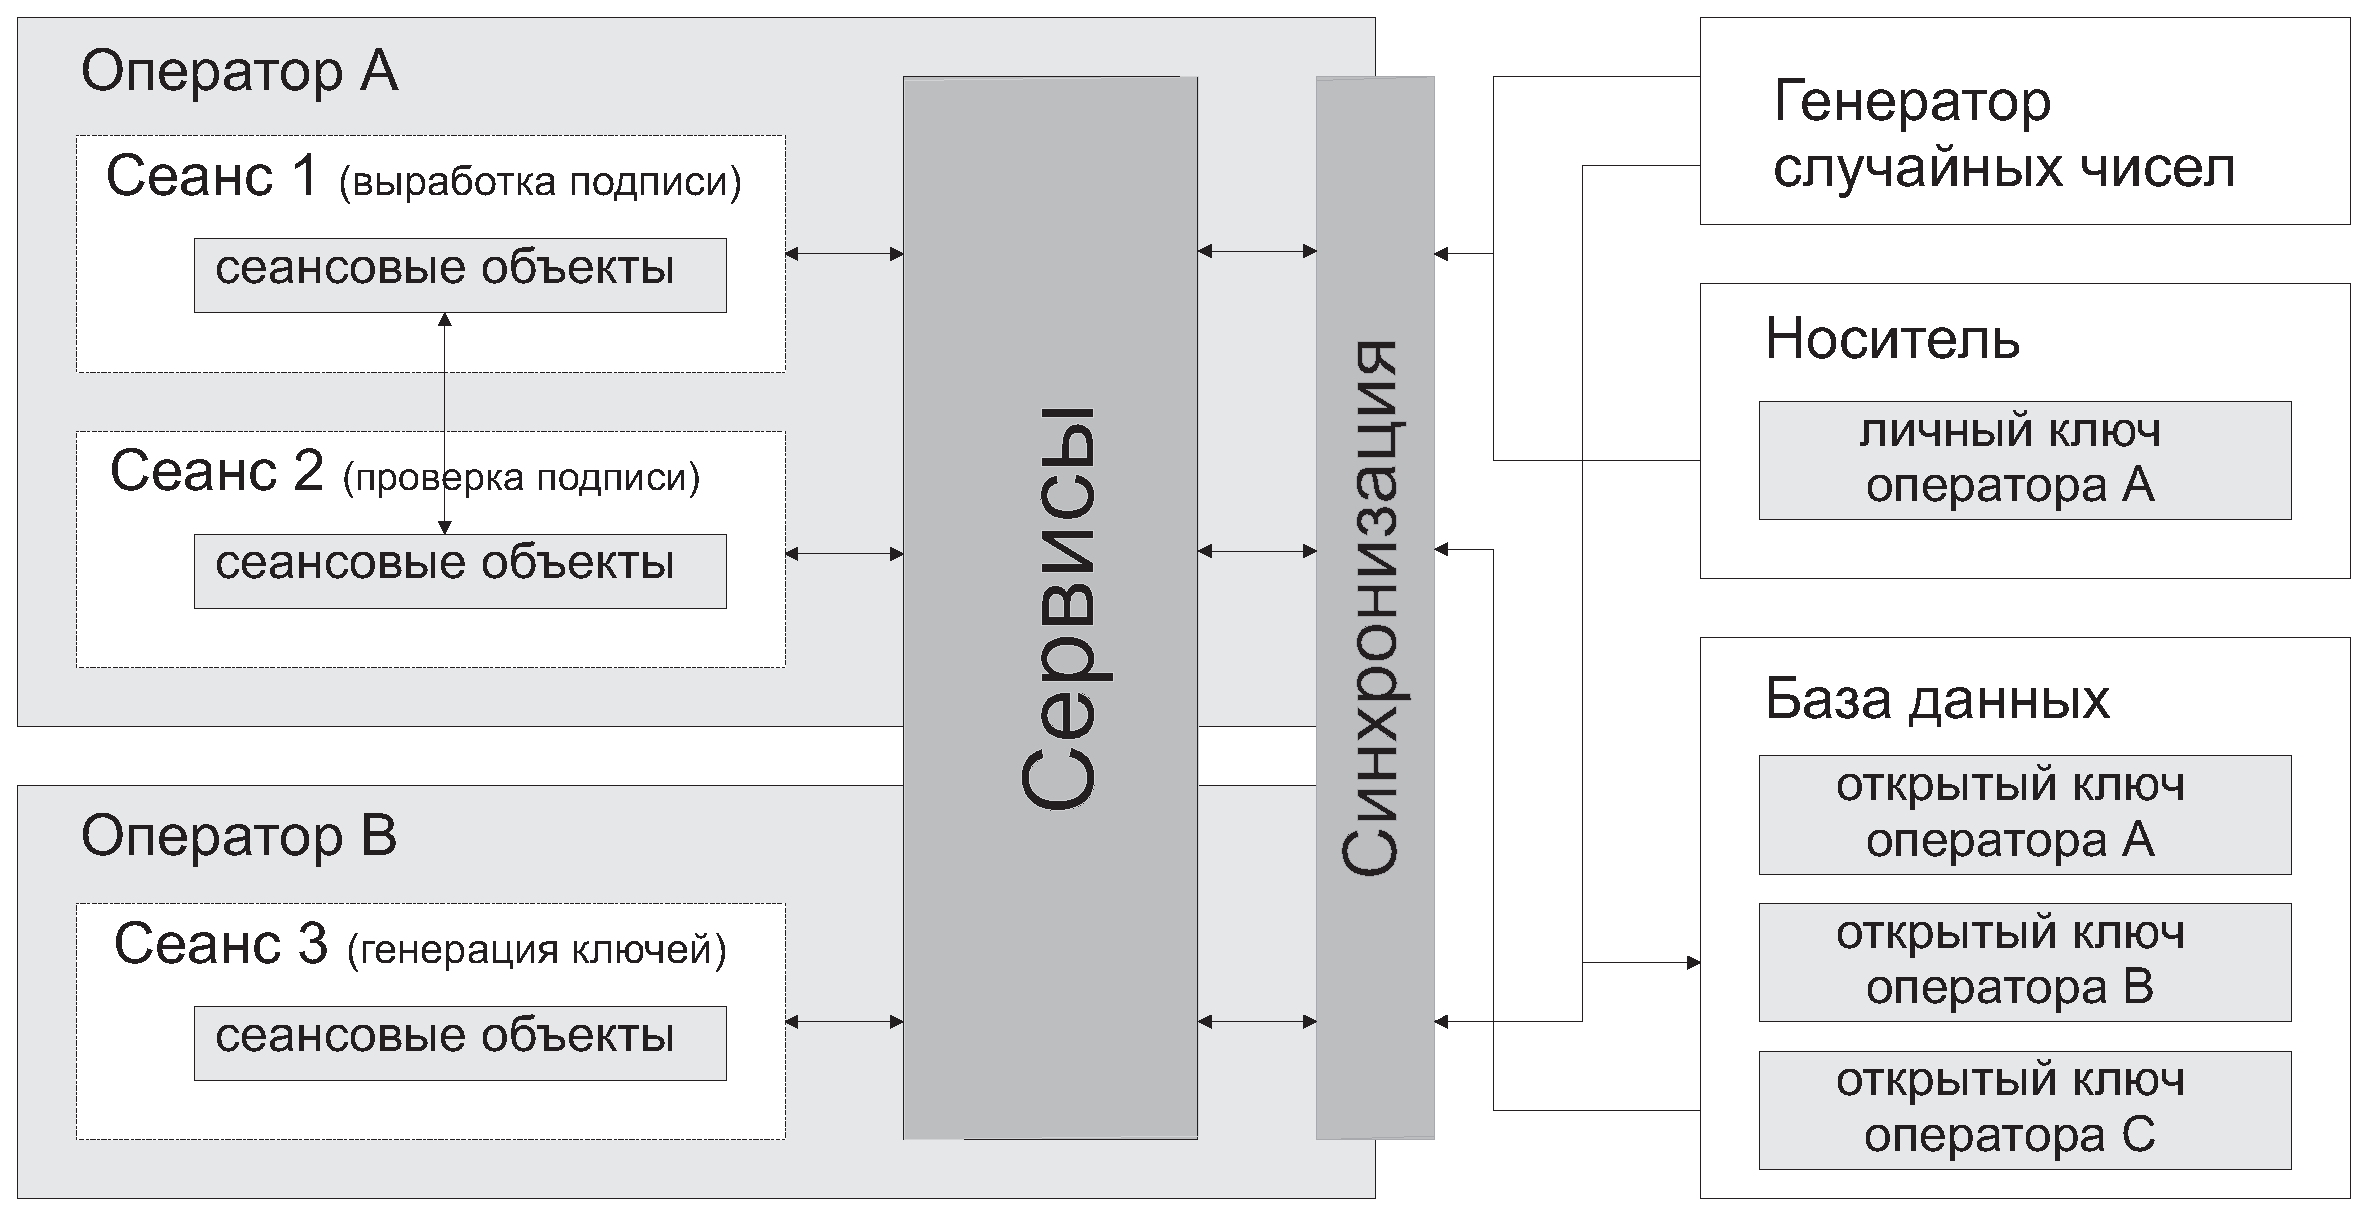
\epsfig{file=Session.eps,width=13cm}
%\end{center}
%\caption{Сеансы и объекты}\label{Fig.Descr.Session}
%\end{figure}

Обращения операторов, прошедших аутентификацию, к сервисам и объектам~\TOE 
регулируются политикой управления доступом. 
Политика регламентирует набор допустимых 
операций операторов над сервисами и объектами.
%
Список разрешенных операций определяется идентификатором и ролью 
оператора, типом объекта, владельцем объекта, 
состоянием, в котором находится сеанс оператора, и другими условиями.
%
Список операций может включать: 
выполнение сервисов,
создание,
удаление,
экспорт,
импорт,
чтение, 
запись объектов~\forref{DAC}.

\section{Защита объектов}

Сеансовый объект может быть преобразован в долговременный,
\ie может экспортироваться за пределы сеанса.
%
При экспорте сеансовые объекты защищаются, \ie обеспечивается
\begin{itemize}
\item[--]
конфиденциальность критических объектов;
\item[--]
контроль целостности открытых и критических объектов.
\end{itemize}

%Экспортом не считается передача объекта во владение другому сеансу доверенного
%СКЗИ в криптографической границе. 
%%
%Рассмотрим пример. Пусть в некотором ПСКЗИ 
%реализован сервис генерации случайных чисел.
%Сервис вызывает другое ПСКЗИ и использует 
%случайные числа для создания ключа, 
%который затем сохраняется на смарт-карте.
%%
%Случайные числа являются критическим сеансовым объектом первого средства
%и передаются во владение второму. 
%Личный ключ является критическим сеансовым объектом второго средства
%и экспортируется на смарт-карту.

%
%Защита критических объектов выполняется непосредственно
%при экспорте средствами~\TOE.
%%
%Защита открытых объектов и частичных секретов 
%выполняется либо непосредственно 
%при экспорте средствами~\TOE, либо позже средствами доверенных~СКЗИ.
%%
%В последнем случае ответственность за отложенную защиту возлагается
%на среду экcплуатации.

Обратно долговременные объекты могут импортироваться из-за 
пределов сеанса. При импорте проверяется целостность 
объектов и дополнительно критические объекты преобразуются 
из защищенной формы в открытую, например расшифровываются.

Для защиты объектов используются следующие методы:

1~{\it Криптографические методы}. 
Состоят в применении алгоритмов шифрования 
(блочного, поточного, с открытым ключом)
для обеспечения конфиденциальности,
алгоритмов ЭЦП и имитозащиты для контроля 
целостности~\forref{DPTCryptoEncr},
\forref{DPTCryptoIntegrity}.

2~{\it Аппаратные методы}. 
Состоят в аппаратной защите от несанкционированного
чтения и (или) модификации областей памяти,
в которых размещаются целевые объекты.
Аппаратная защита обеспечивается применением смарт-карт, токенов
и других подобных устройств~\forref{DPTHard}. 

%Tamper-Resistant Security Module (TRSM) must
%meet the requirements of a Physically Secure Device
%as defined in ISO 9564-1. Such a device must have a
%negligible probability of being successfully penetrated
%to disclose all or part of any secret or private
%cryptographic key or PIN. A TRSM can be so certified
%only after it has been determined that the device’s
%internal operation has not been modified to allow
%penetration (e.g., the insertion within the device of an
%active or passive “tapping” mechanism).

3~{\it Методы разделения секрета}. 
Состоят в разбиении защищаемого критического объекта на частичные секреты, 
каждый из которых затем защищается по отдельности.
%
Простейшим методом разделения секрета является представление
ключа как двоичного слова в виде суммы (поразрядной по модулю $2$)
нескольких частичных секретов. 
В этом случае для восстановления исходного 
ключа требуется располагать всеми частичными секретами.
%
Более сложные пороговые методы позволяют 
определить исходный ключ при наличии не всех, 
а только порогового числа частичных секретов, 
например трех из пяти~\forref{DPTSplit}.

4~{\it Алгоритмические методы}. 
Состоят в контроле целостности с помощью некриптографических или 
бесключевых криптографических алгоритмов.
К алгоритмическим методам относятся: 
сверка нескольких копий объекта, 
проверка контрольных хэш-значений,
самоподпись сертификата открытого ключа~\forref{DPTAlgo}.

5~{\it Организационные меры}. 
Состоят в обеспечении конфиденциальности с помощью мероприятий,
не относящихся к информационным технологиям.

При выборе методов защиты предпочтение следует отдавать 
криптографическим методам. Однако для организации криптографической защиты 
объектов при экспорте и импорте требуется использовать другие 
объекты-ключи. Если эти объекты также нужно экспортировать или 
импортировать, то для их защиты должны использоваться новые ключи
и т.~д. Аппаратные методы и методы разделения секрета позволяют
прервать цепочку ключей защиты других ключей.

В алгоритмических методах защиты контрольная характеристика, 
на основании которой принимается решение о целостности объекта, 
может не защищаться и храниться вместе с самим объектом.
Тогда алгоритмический метод обеспечивает защиту только от случайных сбоев 
в среде эксплуатации, но не от преднамеренного воздействия. 
%
Если же контрольная характеристика защищается, то защита распространяется
на контролируемый объект. 
%
Пусть, например, \TOE вырабатывает личный и открытый ключи,
сохраняет личный ключ на смарт-карту, 
а открытый ключ отсылает в удостоверяющий центр для получения сертификата. 
%
После получения сертификата \TOE вычисляет по сохраненному личному ключу 
открытый и сравнивает его с ключом, размещенным в сертификате.
%
Проверка связи между ключами соответствует алгоритмическому методу защиты.
Аппаратная защита личного ключа распространяется в момент импорта
на открытый ключ сертификата. 

Защита критических сеансовых объектов включает невозможность 
их определения после завершения сеансов.
Для очистки сеансовых объектов в оперативной памяти можно использовать 
обнуление ячеек памяти,
а для очистки объектов в постоянной перепрограммируемой памяти 
может быть использована многократная перезапись ячеек 
константами и случайными данными~\forref{DPTZeroization}.

\section{Среда эксплуатации}

Для учета возможных уязвимостей в среде эксплуатации 
разработчик определяет криптографическую границу~---
непрерывный физический периметр, 
который задает контролируемую границу~\TOE.

В криптографической границе~\TOE выделяются
критические системные компоненты~--- 
аппаратное и программное обеспечение, которое используется
для передачи, обработки и хранения объектов~\TOE.
%(рисунок~\ref{Fig.Descr.TOE}).
К критическим системным компонентам относятся:
\begin{itemize}
\item[--]
устройства ввода/вывода;

\item[--]
устройства обработки и передачи (процессор, физические интерфейсы);

\item[--]
устройства хранения (жесткий диск);

\item[--]
службы операционной системы, влияющие на безопасность~\TOE;

\item[--]
дополнительное оборудование (генераторы случайных чисел).
\end{itemize}

%\begin{figure}[bht]
%\begin{center}
%\epsfig{file=TOE.eps,width=13cm}
%\end{center}
%\caption{\doubt{Среда эксплуатации}}\label{Fig.Descr.TOE}
%\end{figure}

\TOE не может обеспечить безопасность критических системных компонентов,
обеспечение безопасности возлагается на среду.
%
Перед установкой и использованием~\TOE производится настройка среды. 
При настройке конфигурируются средства защиты операционной системы, 
задаются разрешения на установку программ, 
вводятся ограничения на доступ к системным объектам и др.

В~\TOE предусматриваются средства проверки  
условий безопасности среды, 
направленные на контроль состава и правильного 
функционирования критических компонентов.
%
Проверки могут быть косвенными. 
Например, успешная загрузка операционной системы
может являться основанием для вывода о корректности работы
устройств обработки и запоминающих устройств.
В свою очередь проверка
операционной системы может заключаться в контроле версий ее модулей.
%
В большинстве случаев нельзя провести исчерпывающее тестирование 
критических системных компонентов. Допускается, что при тестировании 
проверяется только их наличие и проводится контроль лишь нескольких 
их основных функций.
%
Для некоторых компонентов при начальном запуске можно провести лишь часть 
проверок. В таких случаях разрешается выполнить пропущенные тесты позднее.
Например, при начальном запуске проверяется
наличие устройства чтения смарт-карт, 
а корректность работы данного устройства проверяется 
при непосредственном чтении данных с карты~\forref{CSCTests}.

При обработке объектов~\TOE в критических системных компонентах
могут появляться побочные каналы, по которым передается информация
о критических объектах. 
%
Например, алгоритм выработки ЭЦП может быть реализован таким образом,
что по времени его выполнения нарушитель может сделать вывод 
о значении некоторых битов личного ключа~\forref{CryptoTiming}. 

Побочным каналом является канал сохранения неявных 
копий сеансовых объектов в файле подкачки, регистрах процессора, 
журнале аудита~\forref{LeakProtect}.

В~\TOE второго класса предусматриваются средства защиты от побочных каналов.

\section{Генерация случайных чисел}

В криптографической границе \TOE могут находиться генераторы случайных
чисел, которые вырабатывают данные для создания 
секретных и личных ключей, синхропосылок, других критических или 
уникальных объектов.
К генераторам случайных чисел не относятся 
алгоритмы выработки псевдослучайных чисел,
хотя ключи таких алгоритмов могут строиться с помощью генераторов.

Генератор случайных чисел выдает последовательности,
каждый следующий элемент которых 
статистически и вычислительно трудно предсказать 
по всем предыдущим элементам.
%
Генератор использует один или несколько 
источников случайности (неопределенности, энтропии)
и включает средства обработки данных от источников. 
%
Средства обработки могут частично или полностью 
размещаться в~\TOE~\forref{RNG}.

В компьютерных системах 
используются следующие источники случайности~\forref{RNG}:
\begin{itemize}
\item[--]
физические источники, использующие процессы в физических устройствах
(например, шум в радиоэлектронных приборах);

\item[--]
системные источники, использующие состояния, 
процессы и события операционной системы
(системное время, сетевая активность, прерывания);

\item[--]
источники, основанные на активности операторов
(движения мышью, нажатия клавиш).
\end{itemize}

Предпочтительным является использование физических источников случайности.

Для источника случайности $S$ проводится оценка энтропии 
(неопределенности, вариабельности) его выходных последовательностей.
Для этого строится вероятностная модель~$S$ 
и в рамках этой модели определяется величина~$h$ такая, 
что основная вероятностная масса выходных последовательностей 
длины~$n$ сосредоточена на множестве мощности~$2^{nh}$.
Величина~$h$ называется удельной энтропией на наблюдение.
%
Например, если~$S$ выдает случайные независимые символы 
алфавита~$A$ и вероятность появления символа~$\alpha$ 
равняется~$p_\alpha$, то удельная энтропия
$$
h=-\sum_{\alpha\in A}p_\alpha\log_2 p_\alpha\quad
(0\cdot\log_2 0=0).
$$

Кроме~$h$ существуют и другие характеристики неопределенности,
в частности минимальная удельная энтропия~$h_{min}$,
которая характеризует сложность предсказания самой 
вероятной выходной последовательности~$S$.
Для описанного выше источника величина~$h_{min}$
определяется как~$\min_{\alpha\in A}(-\log_2 p_\alpha)$.

Оценка~$h$ (или $h_{min}$) является сложной задачей, 
если распределение $\{p_\alpha\}$ известно не полностью,
источник~$S$ не является стационарным,
между выходными символами~$S$ имеются зависимости и в других ситуациях.
%
Для оценки~$h$ могут применяться статистические методы,
основанные на частотах встречаемости в выходных последовательностях
$m$-грамм, а также алгоритмические методы, основанные на коэффициентах 
обратимого или необратимого сжатия выходных 
последовательностей~\forref{Entropy}.

Если удельная энтропия $h$ оценена, то можно сделать вывод о том, что для 
надежной генерации $l$-битового секретного ключа требуется использовать 
не менее $l/h$ наблюдений от источника случайности~\forref{Entropy}.

Для выявления отказов и сбоев в функционировании физических источников 
случайности при генерации критических объектов проводится тестирование
выходных последовательностей генераторов случайных чисел. 
Тестирование может быть статистическим~\forref{RNGTests}. 


\input{6FReqsTOE}
\chapter{Функциональные требования безопасности к среде}\label{FReqsEnv}

\section{Требования по идентификации и аутентификации (ИА)}

\req{ИА}{1, 2}\label{Identification}
Каждому оператору должен быть назначен идентификатор и набор 
ролей~\useref{Roles}.

\req{ИА}{1, 2}\label{AuthData}
Для каждого идентификатора оператора~\useref{Identification}
должны быть определены аутентификационные данные. 
Среди аутентификационных данных должны быть выделены 
секреты аутентификации.
%
Устройства ввода аутентификационных данных 
должны быть включены в список критических системных 
компонентов~\forref{CSCList}.

\req{ИА}{1, 2}\label{Authentication}
Должны быть определены и корректно реализованы средства 
аутентификации для проверки 
подлинности идентификатора оператора и возможности выполнения 
оператором сервисов соответствующих ролей~\useref{DAC}.
%
Средства аутентификации, реализуемые~\TOE, 
должны быть включены в список сервисов~\forref{Services}.

\req{ИА}{2}\label{Auth2Factor}
Должно использоваться не менее двух факторов аутентификации.

\req{ИА}{1, 2}\label{AuthStrength}
Вероятность пройти аутентификацию, 
не зная секретов аутентификации, 
не должна превышать~$10^{-6}$, 
если предпринимается одна попытка аутентификации, 
и не должна превышать $10^{-5}$, 
если предпринимаются попытки в течение $1$~мин.

\req{ИА}{1, 2}\label{PwdMask}
Информация, которая отображается при вводе секретов аутентификации, 
не должна ослаблять стойкость средств аутентификации.

\req{ИА}{1, 2}\label{PwdSet}
Должны быть определены и реализованы средства проверки качества 
секретов аутентификации. 
Средства должны применяться при каждой установке или смене секрета.

\req{ИА}{1, 2}\label{AuthSecrets}
При реализации средств аутентификации в~\TOE
контрольные значения аутентификационных данных 
должны быть отнесены к открытым объектам~\forref{Objects}.
Контрольные значения секретов аутентификации
должны быть отнесены к критическим объектам~\forref{Objects}.
Сеансовые объекты, которые содержат значения секретов аутентификации,
также должны быть отнесены к критическим объектам~\forref{Objects}.

\section{Требования по настройке среды (НС)}

\req{НС}{1, 2}\label{ENVInstall}
Должны быть определены настройки среды эксплуатации
для безопасной установки~\TOE уполномоченным администратором.

\req{НС}{1, 2}\label{ENVObjects}
Должны быть определены настройки среды эксплуатации
для обеспечения целостности долговременных объектов~\useref{Objects} 
при их хранении внутри криптографической границы. 
Выбранные настройки должны предотвращать 
изменение долговременных объектов вне сеансов между операторами и~\TOE.

\req{НС}{1, 2}\label{ENVSession}
Должны быть определены настройки среды эксплуатации
для обеспечения конфиденциальности и целостности 
сеансовых объектов~\useref{Objects}  
и аутентификационных данных при их передаче и обработке 
в критических системных компонентах во время сеансов операторов.



\chapter{Гарантийные требования безопасности}\label{AReqs}

\section{Требования по проектированию и разработке (ПР)}

\req{ПР}{1, 2}\label{ProgSpec}
Должно быть дано описание программ~\TOE и установлено соответствие 
между функциональной спецификацией и средствами безопасности,
реализованными в программах.

\req{ПР}{1, 2}\label{HLD}
В описании программ~\useref{ProgSpec}
должны быть определены все внешние интерфейсы~\TOE.

\req{ПР}{2}\label{LLD}
В описании программ~\useref{ProgSpec}
должны быть определены внутренние компоненты~\TOE и их интерфейсы.

\req{ПР}{1, 2}\label{Tools}
В описании программ~\useref{ProgSpec}
должны быть определены все используемые средства разработки
и сборки программ. Должны быть перечислены все конфигурационные файлы,
отвечающие за настройку средств разработки и сборки. 
Конфигурационные файлы должны быть включены в список 
элементов конфигурации~\forref{CMList}.

\req{ПР}{1, 2}\label{Comments}
Исходные тексты программ должны быть снабжены комментариями,
устанавливающими соответствие с описанием программ~\forref{ProgSpec}.

\req{ПР}{1, 2}\label{Language}
Программы должны быть написаны на высокоуровневых языках программирования.
Вставки на низкоуровневых языках (языках ассемблера)
допускаются в случаях, критичных для производительности, 
а также тогда, когда высокоуровневые языки применить нельзя.


\section{Требования по поддержке жизненного цикла (ЖЦ)}

\req{ЖЦ}{1, 2}\label{CMSystem}
Должна быть определена и реализована система управления конфигурацией для \TOE.
Система должна обеспечивать:
\begin{itemize}
\item[--]
контроль доступа разработчиков к элементам конфигурации;
\item[--]
контроль версий элементов конфигурации;
\item[--]
отслеживание изменений элементов конфигурации;
\item[--]
сборку программ по исходным текстам~\useref{Tools}.
\end{itemize}

\req{ЖЦ}{1, 2}\label{CMList}
В перечень элементов конфигурации должны быть включены:
\begin{itemize}
\item[--]
функциональная спецификация;
\item[--]
программы;
\item[--]
описание программ~\useref{ProgSpec};
\item[--]
исходные тексты программ;
\item[--]
документация по управлению конфигурацией~\useref{CMSystem};
\item[--]
документация по поставке~\TOE потребителю~\useref{Delivery};
\item[--]
документация по устранению недостатков~\useref{FlawRemediation}
(только для класса 2);
\item[--]
руководства~\useref{AdminGuide}, \useref{UserGuide}.
\end{itemize}

\req{ЖЦ}{1, 2}\label{CMVersion}
Каждая версия каждого элемента конфигурации 
должна быть снабжена уникальным идентификатором. 

\req{ЖЦ}{1, 2}\label{Delivery}
Должна быть определена и реализована система поставки~\TOE потребителю.  

\req{ЖЦ}{2}\label{Authenticode}
Должны быть предусмотрены средства контроля целостности и подлинности 
инсталляционных программ после их доставки потребителю. 

\req{ЖЦ}{2}\label{FlawRemediation}
Должна быть определена и реализована система устранения недостатков 
в программах и документации~\TOE.
Система должна обеспечивать:
\begin{itemize}
\item[--]
регистрацию недостатков;
\item[--]
определение порядка выявления причин недостатков
и исправления недостатков;
\item[--]
отслеживание статуса недостатков 
(подтвержден, исправляется, исправлен и др.);
\item[--]
описание способа устранения недостатков;
\item[--]
порядок извещения потребителей об устранении недостатков.
\end{itemize}

\section{Требования к руководствам (РД)}

\req{РД}{1, 2}\label{AdminGuide}
Должно быть разработано руководство администратора.
Руководство должно описывать:
\begin{itemize}
\item[--]
обязанности администратора по настройке среды~\useref{ENVInstall}, 
\useref{ENVObjects}, \useref{ENVSession};
\item[--]
инструкции по установке~\TOE~\useref{ENVInstall};
\item[--]
доступные администратору сервисы~\useref{DAC};
\item[--]
обязанности администратора по настройке средств безопасности~\TOE;
\item[--]
связанные с безопасностью предположения 
относительно поведения операторов.
\end{itemize}

\req{РД}{1, 2}\label{UserGuide}
Для каждой роли~\useref{Roles}, отличной от роли <<Администраторы>>, 
должно быть разработано руководство ее операторов.
Руководство должно определять:
\begin{itemize}
\item[--]
доступные оператору сервисы~\useref{DAC};
\item[--]
обязанности оператора по обеспечению безопасности~\TOE.
\end{itemize}

\req{РД}{2}\label{Misuse}
Руководства~\useref{AdminGuide}, \useref{UserGuide} 
должны описывать типичные ошибки операторов,
которые могут привести к снижению безопасности~\TOE.
Руководства должны давать рекомендации операторам по избежанию
ошибок.

\section{Требования по программе испытаний (ПИ)}

\req{ПИ}{1, 2}\label{TestProgram}
Должна быть разработана программа испытаний~\TOE разработчиком.
Программа должна определять:
\begin{itemize}
\item[--]
планы тестирования;
\item[--]
содержание тестов;
\item[--]
ожидаемые результаты выполнения тестов;
\item[--]
фактические результаты выполнения тестов.
\end{itemize}

\req{ПИ}{1, 2}\label{TestCoverage}
Тесты программы испытаний~\useref{TestProgram} должны 
покрывать все функциональные возможности~\TOE, 
определенные в функциональной спецификации.

\req{ПИ}{2}\label{TestDeep}
Тесты программы испытаний~\useref{TestProgram} должны 
покрывать функциональные возможности всех компонентов~\TOE, 
определенных в описании программ~\useref{ProgSpec}.



\begin{appendix}{А}{рекомендуемое}
{Содержание функциональной спецификации}
\label{SPEC}

\mbox{}

\begin{enumerate}
\item
{Описание~\TOE.}

\begin{enumerate}
\item
Назначение.
\item
Класс ($1$ или $2$).
\item
Основные функциональные возмножности.
\item
Криптографическая граница.
\item
Список критических системных компонентов~\useref{CSCList}.
\end{enumerate}

\item
{Криптографическая поддержка.}

\begin{enumerate}
\item
Список криптографических алгоритмов и протоколов~\useref{CryptoAlg}.

\item
Методы генерации долговременных параметров и ключей~\useref{CryptoGen}.

\item
Средства контроля времени выполнения криптографических алгоритмов 
и протоколов~\useref{CryptoTiming} (только для класса 2).
\end{enumerate}

\item
{Реализация сервисов.}
\begin{enumerate}
\item
Список сервисов~\useref{Services}.

\item
Средства защиты от создания неявных копий
критических объектов~\useref{LeakProtect} 
(только для класса 2).
\end{enumerate}

\item
{Управление доступом.}

\begin{enumerate}
\item
Список ролей операторов~\useref{Roles}.

\item
Список объектов~\useref{Objects}.

\item
Описание политики управления доступом~\useref{DAC}.

\item
Состояния системного сеанса и правила перехода между состояниями~\useref{States}.
\end{enumerate}

\item
{Защита объектов.}

\begin{enumerate}
\item
Криптографические методы обеспечения конфиденциальности~\useref{DPTCryptoEncr}.

\item
Криптографические методы контроля целостности~\useref{DPTCryptoIntegrity}.

\item
Аппаратные методы защиты~\useref{DPTHard}.

\item
Методы разделения секрета~\useref{DPTSplit}.

\item
Алгоритмические методы контроля целостности~\useref{DPTAlgo}.

\item
Организационные методы обеспечения конфиденциальности~\useref{DPTOrg}.

\item
Соответствие <<объекты~--- методы защиты>>~\useref{DPTCrit}, \useref{DPTPublic}.

\item
Методы очистки критических сеансовых объектов~\useref{DPTZeroization}.
\end{enumerate}

\item
{Самотестирование.}

\begin{enumerate}
\item
Проверка работоспособности критических системных компонентов~\useref{CSCTests}.

\item
Перечень проверок самотестирования~\useref{SelfTests}.

\item
Обработка ошибок тестирования~\useref{TestLock}.
\end{enumerate}

\item
{Генерация случайных чисел.}

\begin{enumerate}
\item
Описание генераторов случайных чисел~\useref{RNG}.

\item
Оценка энтропии источников случайности~\useref{Entropy}.

\item
Тестирование выходных последовательностей генераторов~\useref{RNGTests}.
\end{enumerate}

\item
{Идентификация и аутентификация.}

\begin{enumerate}
\item
Методы идентификации операторов~\useref{Identification}.

\item
Методы аутентификации операторов~\useref{AuthData}, \useref{Authentication}.

\item
Проверка качества секретов аутентификации~\useref{PwdSet}.
\end{enumerate}

\item
{Настройка среды.}

\begin{enumerate}
\item
Настройка среды для безопасной установки~\useref{ENVInstall}.

\item
Настройка среды для защиты системных объектов~\useref{ENVObjects}.

\item
Настройка среды для защиты сеансов~\useref{ENVSession}.
\end{enumerate}

\item
Гарантийные меры (могут быть определены в отдельных документах).
\begin{enumerate}
\item
Описание программ~\useref{ProgSpec}.

\item
Внешние интерфейсы программ~\useref{HLD}.

\item
Внутренние компоненты и интерфейсы~\useref{LLD}
(только для класса 2).

\item
Cредства разработки~\useref{Tools}.

\item
Языки программирования~\useref{Language}.

\item
Система управления конфигурацией~\useref{CMSystem}.

\item
Система поставки~\TOE потребителю~\useref{Delivery}.

\item
Методы контроля инсталляционных программ~\useref{Authenticode}
(только для класса 2).

\item
Список руководств~\useref{AdminGuide}, \useref{UserGuide}.

\item
Типичные ошибки операторов~\useref{Misuse}
(только для класса 2).

\item
Программа испытаний~\useref{TestProgram}.

\item
Результаты анализа покрытия тестами~\useref{TestCoverage}.

\item
Результаты анализа глубины тестирования~\useref{TestDeep}
(только для класса 2).
\end{enumerate}
\end{enumerate}

Допускается объединять разделы.
Если в~\TOE не реализован необязательный механизм безопасности, 
то соответствующий раздел можно опустить.

\end{appendix}


\providecommand{\CryptoKernel}{<<{Криптоядро}>>\xspace}
\begin{appendix}{Б}{справочное}{Программное средство \CryptoDisk 
(примерная спецификация)}
\label{EXAMPLE} 

\hiddensection{Описание}

\paragraph*{Назначение.} 
Программное средство~\CryptoDisk предназначено для шифрования 
файлов на магнитных носителях <<на лету>>. 
%
С помощью программного средства пользователи могут создавать частные каталоги,
при записи в которые файлы будут зашифровываться, 
а при чтении~--- расшифровываться.
%
Сам каталог без обработки~программным средством представляет 
собой обычный файл операционной системы. 
%
Пользователи, которым запрещено чтение каталога,
не могут раскрыть его содержание даже при доступе к данному файлу.

\paragraph*{Класс.} 
\CryptoDisk является средством класса~$2$.

\paragraph*{Основные функциональные возможности.} 
\CryptoDisk реализует:
\begin{itemize}
\item[--]
управление частными каталогами нескольких пользователей;
\item[--]
шифрование файлов каталога <<на лету>>;
\item[--]
хранение ключей на USB-токенах;
\item[--]
возможность записи файлов в каталог 
любым авторизованным пользователем;
\item[--]
установку разрешений на доступ к отдельным файлам 
каталога совместно администратору и выбранному доверенному пользователю 
(на случай утери или блокировки токена владельца).
\end{itemize}

\paragraph*{Криптографическая граница.}
\CryptoDisk выполняется на персональном компьютере. 
Криптографической границей является периметр системного 
блока компьютера.

\paragraph*{Критические системные компоненты.}
В пределах криптографической границы находятся следующие критические 
системные компоненты:

\begin{definition}{CSC.Board}{Вычислительная платформа}
Процессор, материнская плата, устройства хранения, 
порты ввода/вывода и другие аппаратные 
компоненты персонального компьютера, 
необходимые для выполнения программ и хранения данных~\CryptoDisk.
%
Должны быть доступны два порта для USB-токенов.
%
Должен присутствовать высокоточный таймер.
\end{definition}

\begin{definition}{CSC.OS}{Операционная система}
Компоненты операционной системы, 
отвечающие за безопасное выполнение программ~\CryptoDisk. 
Должна использоваться операционная система линейки~Windows.
\end{definition}

\hiddensection{Криптографическая поддержка}\label{EXAMPLE.Crypto}

\paragraph*{Криптографические алгоритмы.} 
В~\CryptoDisk
реализованы следующие криптографические алгоритмы:

\begin{definition}{Alg.DataWrap}{Алгоритмы одновременного шифрования и имитозащиты}
Алгоритмы одновременного шифрования и имитозащиты, определенные в~ТНПА-1. 
Реализованы алгоритм установки защиты 
(зашифрование и вычисление имитовставки) 
и алгоритм снятия защиты
(проверка имитовставки и расшифрование).
Алгоритмы предназначены для защиты файлов в частных каталогах.
\end{definition}

\begin{definition}{Alg.Transport}{Алгоритмы транспорта ключей} 
Алгоритмы транспорта ключей, определенные в ТНПА-2. 
Реализованы алгоритм установки защиты транспортируемого
ключа и алгоритм снятия защиты. 
При установке защиты используется открытый ключ оператора, 
которому транспортируется ключ,
а при снятии защиты используется личный ключ того же оператора.
Алгоритмы предназначены для транспорта ключей~\ref{Alg.DataWrap}.
\end{definition}

\begin{definition}{Alg.Sign}{Алгоритмы ЭЦП} 
Алгоритмы электронной цифровой подписи, определенные в ТНПА-3. 
Реализованы алгоритмы выработки и проверки ЭЦП.
Используется администратором для заверения открытых 
ключей~\ref{Alg.Transport} и пользователями для проверки заверения.
\end{definition}

\begin{definition}{Alg.PRNG}{Алгоритм генерации псевдослучайных чисел} 
Алгоритм генерации псевдослучайных чисел с секретным параметром, 
определенный в ТНПА-4. 
Алгоритм предначен для генерации ключей~\ref{Alg.DataWrap} и~\ref{Alg.Transport}, 
других случайных параметров криптографических алгоритмов.
\end{definition}

\begin{definition}{Alg.Hash}{Алгоритм хэширования} 
Алгоритм хэширования, определенный в ТНПА-5. 
Алгоритм предначен для вычисления контрольных характеристик 
системных объектов. Является композиционным 
элементом~\ref{Alg.Transport} и~\ref{Alg.Sign}.
Используется в генераторе случайных чисел.
\end{definition}

\paragraph*{Генерация ключей и параметров.} 
Алгоритмы~\ref{Alg.DataWrap}, \ref{Alg.PRNG} и \ref{Alg.Hash}
не имеют долговременных параметров. 
%
Долговременные параметры~\ref{Alg.Transport} и~\ref{Alg.Sign} совпадают.
К ним относятся параметры эллиптической кривой и базовая точка на ней. 
Эти параметры генерируются по алгоритму, определенному в ТНПА-3, 
фиксируются в программах~\CryptoDisk и используются всеми операторами.

Ключ~\ref{Alg.PRNG} вырабатывается с помощью генератора случайных чисел~(Б.7). 
После создания ключ записывается на токен вместе с нулевым счетчиком. 
Дальнейшая работа с~\ref{Alg.PRNG} регулируется следующими правилами:
\begin{enumerate} 
\item
При обращении к~\ref{Alg.PRNG} ключ и счетчик читаются с токена. 
По ним вырабатываются псевдослучайные данные требуемого объема. 
\item
При выработке данных счетчик изменяется.
Новое значение счетчика записывается на токен. 
\item
Если запись прошла успешно,
то сформированные псевдослучайные данные используются по назначению. 
В противном случае данные уничтожаются 
и обращение к~\ref{Alg.PRNG} завершается ошибкой.
\end{enumerate} 

По данным правилам вырабатываются 
секретные ключи и синхропосылки~\ref{Alg.DataWrap}, 
личные ключи и секретные параметры~\ref{Alg.Transport} и~\ref{Alg.Sign},
частичные секреты и др.

\clearpage

Открытые ключи~\ref{Alg.Transport} и~\ref{Alg.Sign} 
вырабатываются по личному ключу в соответствии с алгоритмами, 
определенными в~ТНПА-2, ТНПА-3.

\paragraph*{Контроль времени выполнения.} 
Алгоритмы~\ref{Alg.DataWrap} и \ref{Alg.PRNG} относятся к классу симметричных.
Время их выполнения не зависит от значений ключей.

Алгоритм~\ref{Alg.Hash} является бесключевым.
При хэшировании объектов, которые могут оказаться критическими, 
время хэширования не зависит от значения объекта
и определяется только размером объекта.

В алгоритмах~\ref{Alg.Transport}, \ref{Alg.Sign}
определяются кратные 
$uP=P+P+\ldots+P$, где $P$~--- точка эллиптической кривой,
которая суммируется $u$ раз.
При этом кратность~$u$ может являться личным ключом 
или одноразовым секретным параметром.
%
Для определения кратных точек используется 
алгоритм <<лестница Монтгомери>> (Montgomery ladder),
время работы которого не зависит от кратности.

\hiddensection{Реализация сервисов}

\paragraph*{Сервисы.} 
\CryptoDisk реализует следующие сервисы:

\begin{definition}{S.GetVersion}{Номер версии}
Сервис отображает номер версии программ в формате 
<<старший номер, младший номер, номер сборки>>. 
\end{definition}

\begin{definition}{S.SelfTest}{Самотестирование}
Сервис самотестирования.
\end{definition}

\begin{definition}{S.InitToken}{Инициализация токена}
На вход сервиса подается идентификатор оператора,
которому токен передается во владение.
%
Сервис настраивает файловую систему токена,
записывает на токен идентификатор и служебные данные.
%
Если оператор не является администратором, 
то дополнительно используется уже инициализированный токен администратора,
%
с которого переписывается ключ~\ref{R.SignKeyPublic}. 
\end{definition}

\begin{definition}{S.GenUserKeys}{Генерация ключей пользователя}
Сервис запрашивает PIN-код доступа и задает его для токена.
После этого для доступа к объектам токена требуется предъявить PIN-код.
%
Сервис генерирует ключи~\ref{R.KeyPRNG}, 
формирует нулевой счетчик~\ref{R.CounterPRNG}
и записывает эти объекты на токен. 
Затем генерируются и записываются на токен ключи~\ref{R.TransportKeyPrivate}
и~\ref{R.TransportKeyPublic}.
%
Ключ~\ref{R.TransportKeyPublic} дополнительно записывается 
в каталог администратора вместе с идентификатором владельца токена.
\end{definition}

\begin{definition}{S.GenAdminKeys}{Генерация ключей администратора}
Сервис выполняет те же действия, что и~\ref{S.GenUserKeys}.
Дополнительно генерируются и записываются на токен ключи~\ref{R.SignKeyPrivate}
и~\ref{R.SignKeyPublic}. Дополнительно вызывается 
сервис~\ref{S.SignTransportKey}, на вход которого подаются
ключ~\ref{R.TransportKeyPublic} и идентификатор администратора.
\end{definition}

\clearpage
\begin{definition}{S.AuthToken}{Аутентификация для доступа к токену}
На вход сервиса подается PIN-код оператора.
PIN-код передается управляющей программе токена. 
После подтверждения PIN-кода оператору разрешается доступ к объектам токена.
\end{definition}

\begin{definition}{S.SignTransportKey}{Подпись ключа транспорта}
На вход сервиса подается запись,
содержащая ключ~\ref{R.TransportKeyPublic}
и идентификатор его владельца.
%
Используется токен администратора.
%
Сервис читает с токена ключ~\ref{R.SignKeyPrivate},
вычисляет на нем ЭЦП записи и добавляет запись вместе с ЭЦП 
в общедоступный справочник открытых ключей.
\end{definition}

\begin{definition}{S.WriteFile}{Запись файла}
На вход сервиса подается файл, который пользователю~$U$
требуется записать в каталог пользователя~$H$.
%
Используется токен~$U$.
Из справочника открытых ключей читается запись,
содержащая идентификатор~$H$ и его ключ~\ref{R.TransportKeyPublic}.
ЭЦП этой записи проверяется на ключе~\ref{R.SignKeyPublic},
который читается с токена~$U$. 
Если проверка прошла успешно, 
то генерируется ключ~\ref{R.DataKey} и на нем устанавливается 
защита входного файла.
%
Ключ~\ref{R.DataKey} защищается на ключе~\ref{R.TransportKeyPublic}
пользователя~$U$ и сохраняется вместе с зашифрованным файлом в каталоге. 
\end{definition}

\begin{definition}{S.ReadFile}{Чтение файла}
На вход сервиса подается зашифрованный файл из частного каталога
и зашифрованный ключ~\ref{R.DataKey} его защиты. 
%
Используется токен владельца каталога.
%
С токена читается ключ~\ref{R.TransportKeyPrivate}
и на нем снимается защита с ключа~\ref{R.DataKey}.
Затем на ключе~\ref{R.DataKey} снимается защита с зашифрованного файла.
\end{definition}

\begin{definition}{S.ShareFile}{Открытие доступа к файлу}
На вход сервиса подается зашифрованный ключ~\ref{R.DataKey},
который хранится вместе с зашифрованным файлом в частном каталоге,
и идентификатор доверенного пользователя, которому совместно с администратором 
предоставляется доступ к файлу.
%
Используется токен владельца каталога.
%
С токена читается ключ~\ref{R.TransportKeyPrivate}
и на нем снимается защита с ключа~\ref{R.DataKey}.
Затем ключ~\ref{R.DataKey} разбивается на два частичных 
секрета~\ref{R.DataKeyPartial}.
%
Каждый из секретов защищается на ключах~\ref{R.TransportKeyPublic} 
доверенного пользователя и администратора. 
%
Ключ~\ref{R.TransportKeyPublic} доверенного пользователя 
читается из общедоступного справочника. Перед использованием 
проверяется его ЭЦП.
%
Зашифрованные частичные секреты сохраняются вместе с файлом в каталоге.
\end{definition}

\begin{definition}{S.RecoverFile}{Восстановление файла}
На вход сервиса подается зашифрованный файл из частного каталога
и зашифрованные частичные секреты~\ref{R.DataKeyPartial}
пользователя и администратора, 
которым совместно открыт доступ к файлу в частном каталоге.
Используются токены доверенного пользователя и администратора.
%
С токенов читаются ключи~\ref{R.TransportKeyPrivate}.
На них снимается защита с~\ref{R.DataKeyPartial}. 
По найденным частичным секретам собирается ключ~\ref{R.DataKey}, 
на котором снимается защита с целевого файла.
\end{definition}

Все сервисы возвращают код ошибки или признак успешного завершения.

Сервисы \ref{S.InitToken}, \ref{S.GenAdminKeys}, \ref{S.GenUserKeys}, 
\ref{S.SignTransportKey} обслуживают управление ключами  
и выполняются в следующей последовательности:

\begin{enumerate}
\item
Администратор генерирует свои
ключи, вызывая~\ref{S.InitToken} и~\ref{S.GenAdminKeys}.

\item
По запросу пользователя администратор инициализирует для него токен,
вызывая~\ref{S.InitToken}. Токен передается пользователю.

\item
Пользователь генерирует ключи, вызывая~\ref{S.GenUserKeys}.
Открытый ключ~\ref{R.TransportKeyPublic} 
помещается в каталог администратора.

\item
Администратор с определенной периодичностью просматривает свой каталог
и подписывает новые записи (идентификатор пользователя, 
открытый ключ пользователя), 
вызывая~\ref{S.SignTransportKey}.
При необходимости перед вызовом сервиса администратор 
проверяет соответствие между идентификатором
и открытым ключом, связываясь с пользователем.
\end{enumerate}

\paragraph*{Защита от создания неявных копий критических объектов.}
Неявные копии критических объектов 
могут создаваться в следующих областях памяти:
\begin{itemize}
\item[--]
файл подкачки (\texttt{pagefile.sys}); 
\item[--]
файл спящего режима (\texttt{hiberfile.sys});
\item[--]
отладочные дампы памяти, сохраняемые операционной системой 
при сбоях в программах.
\end{itemize}
В~\CryptoDisk используется специальные функции выделения
оперативной памяти, которые блокируют попадание критических сеансовых объектов
в файл подкачки.
Дополнительно при настройке среды блокируются спящий режим и 
средства создания отладочных дампов памяти.

\hiddensection{Управление доступом}

\paragraph*{Роли.} 
\CryptoDisk поддерживает роли~\anchor{Role.Admins} (<<Администраторы>>)
и \anchor{Role.Users} (<<Пользователи>>).
Группа~\ref{Role.Admins} включает только одного участника.

\paragraph*{Объекты.} 
Обрабатываются следующие объекты:

\begin{definition}{R.File}{Файл}
Файл частного каталога.
Долговременный критический объект.
Принадлежит владельцу каталога.
\end{definition}

\begin{definition}{R.KeyPRNG}{Секретный ключ~ГПСЧ}
Секретный ключ алгоритма~\ref{Alg.PRNG}.
Вырабатывается с помощью генератора случайных чисел.
Хранится на токене. Принадлежит владельцу токена.
\end{definition}

\begin{definition}{R.CounterPRNG}{Счетчик~ГПСЧ}
Счетчик алгоритма~\ref{Alg.PRNG}. Открытый объект.
Первоначально устанавливается в~$0$, при обращениях к~\ref{Alg.PRNG}
последовательно увеличивается. Хранится на токене. 
Принадлежит владельцу токена.
\end{definition}

%\begin{definition}{R.AuthData}{Контрольные аутентификационные данные}
%Контрольная характеристика пароля доступа к токену.
%Долговременный критический объект.
%Результат $1024$-кратного применения~\ref{Alg.Hash} 
%к паролю пользователя, дополненному случайным числом.
%Хранится на токене вместе с использованным случайным числом.
%Принадлежит владельцу токена.
%\end{definition}

\begin{definition}{R.DataKey}{Ключ защиты данных}
Секретный ключ алгоритмов~\ref{Alg.DataWrap} для защиты~\ref{R.File}.
Генерируется с помощью~\ref{Alg.PRNG}.
Хранится вместе с защищенным файлом. 
Принадлежит владельцу~\ref{R.File}.
\end{definition}

\begin{definition}{R.DataKeyPartial}{Частичный ключ защиты данных}
Секретный частичный ключ алгоритмов~\ref{Alg.DataWrap}.
Владельцем является администратор или один из пользователей.
Частичный ключ администратора генерируется с помощью~\ref{Alg.PRNG}.
Частичный ключ пользователя определяется как сумма~\ref{R.DataKey} 
и частичного ключа администратора. 
Хранится вместе с защищенным файлом. 
\end{definition}

\begin{definition}{R.SignKeyPrivate}{Личный ключ ЭЦП}
Личный ключ алгоритма выработки ЭЦП~\ref{Alg.Sign}.
Генерируются с помощью~\ref{Alg.PRNG}.
Хранится на токене администратора. Принадлежит администратору.
\end{definition}

\begin{definition}{R.SignKeyPublic}{Открытый ключ ЭЦП}
Открытый ключ алгоритма проверки ЭЦП~\ref{Alg.Sign}.
Генерируется по личному ключу~\ref{R.SignKeyPrivate}.
Хранится на токене администратора и на токенах пользователей. 
Принадлежит администратору.
\end{definition}

\begin{definition}{R.TransportKeyPrivate}{Личный ключ транспорта}
Личный ключ алгоритма~\ref{Alg.Transport}.
Генерируется с помощью~\ref{Alg.PRNG}.
Хранится на токене. Принадлежит владельцу токена.
\end{definition}

\begin{definition}{R.TransportKeyPublic}{Открытый ключ транспорта}
Открытый ключ алгоритма~\ref{Alg.Transport}.
Генерируется по личному ключу~\ref{R.TransportKeyPrivate}.
Хранится на токене и в общедоступном справочнике открытых ключей. 
Принадлежит владельцу токена.
\end{definition}

\begin{definition}{R.System}{Системные объекты}
Программы, файлы настроек, общедоступный справочник открытых ключей,
данные для тестирования криптографических алгоритмов, флаг блокировки.
Являются открытыми объектами.
Хранятся в пределах криптографической границы.
\end{definition}

\paragraph*{Политика управления доступом.} 
Политика управления доступом определена в таблице~\ref{Table.CryptoDisk.DAC}.
В таблице операции над объектами обозначаются следующим образом:
\texttt{X}~--- выполнение,
\texttt{C}~--- создание,
\texttt{W}~--- запись,
\texttt{R}~--- чтение.
%
Владельцами объектов, над которыми выполняются операции,
в основном являются операторы, вызывающие сервисы. 
%
Исключение составляют системные объекты, а также объекты, 
снабженные надстрочными символами:
$A$~--- объект администратора, $U$~--- объект другого пользователя, 
$H$~--- объект владельца каталога.

\begin{table}[p]
\caption{Политика управления доступом \CryptoDisk}
\label{Table.CryptoDisk.DAC}
\begin{tabular}{|p{5cm}|p{8.7cm}|c|}
\hline
Операторы и сервисы & Объекты & Операции\\
\hline
\hline
\ref{Role.Admins},        & \ref{S.GetVersion} & \texttt{X}\\
\ref{Role.Users}          & \ref{S.SelfTest} & \texttt{X}\\
                          & \ref{S.GenUserKeys} & \texttt{X}\\
                          & \ref{S.AuthToken} & \texttt{X}\\
                          & \ref{S.ReadFile} & \texttt{X}\\
                          & \ref{S.RecoverFile} & \texttt{X}\\
\hline
\ref{Role.Admins}         & \ref{S.InitToken} & \texttt{X}\\
                          & \ref{S.GenAdminKeys} & \texttt{X}\\
                          & \ref{S.SignTransportKey} & \texttt{X}\\
\hline
\ref{Role.Users}          & \ref{S.WriteFile} & \texttt{X}\\
                          & \ref{S.ShareFile} & \texttt{X}\\
\hline
\hline
\ref{S.GetVersion}& \ref{R.System} (данные о версии) & \texttt{R}\\
\hline
\ref{S.SelfTest}& \ref{R.System} (тестовые данные) & \texttt{R}\\
\hline
\ref{S.InitToken} & \ref{R.SignKeyPublic} & \texttt{W}\\
\hline
\ref{S.GenUserKeys}  & \ref{R.KeyPRNG}& \texttt{CW}\\
                     & \ref{R.CounterPRNG}& \texttt{CW}\\
                     & \ref{R.TransportKeyPrivate}& \texttt{CW}\\
                     & \ref{R.TransportKeyPublic}& \texttt{CW}\\
\hline
\ref{S.GenAdminKeys} & \ref{S.GenUserKeys}& \texttt{X}\\
                     & \ref{R.SignKeyPrivate}& \texttt{CW}\\
                     & \ref{R.SignKeyPublic}& \texttt{CW}\\
                     & \ref{S.SignTransportKey}& \texttt{X}\\
\hline
\ref{S.AuthToken}    & --& \\
\hline
\ref{S.SignTransportKey} & \ref{R.TransportKeyPublic}\up{U} & \texttt{RW}\\
                          & \ref{R.SignKeyPrivate} & \texttt{R}\\
\hline
\ref{S.WriteFile} & \ref{R.TransportKeyPublic}\up{H} & \texttt{R}\\
                     & \ref{R.SignKeyPublic}\up{A} & \texttt{R}\\
                     & \ref{R.DataKey}\up{H} & \texttt{CW}\\
                     & \ref{R.File}\up{H} & \texttt{W}\\
\hline
\ref{S.ReadFile}  & \ref{R.File}& \texttt{R}\\
                     & \ref{R.DataKey}& \texttt{R}\\
                     & \ref{R.TransportKeyPrivate}& \texttt{R}\\
\hline
\ref{S.ShareFile} & \ref{R.DataKey}& \texttt{R}\\
                     & \ref{R.TransportKeyPrivate} & \texttt{R}\\
                     & \ref{R.DataKeyPartial}\up{UA} & \texttt{CW}\\
                     & \ref{R.TransportKeyPublic}\up{UA} & \texttt{R}\\
                     & \ref{R.SignKeyPublic}\up{A} & \texttt{R}\\
\hline
\ref{S.RecoverFile} & \ref{R.DataKeyPartial} & \texttt{R}\\
                     & \ref{R.TransportKeyPrivate} & \texttt{R}\\
                     & \ref{R.DataKey}\up{H} & \texttt{C}\\
                     & \ref{R.File}\up{H} & \texttt{R}\\
\hline
\end{tabular}
\end{table}

\paragraph*{Состояния.} 
Главная программа~\CryptoDisk реализует службу операционной системы Windows.
Выполнение службы начинается при запуске системы и заканчивается при ее завершении.
Системный сеанс~\CryptoDisk соответствует периоду выполнения службы.

Используются следующие состояния системного сеанса 
и правила перехода между состояниями:

\clearpage
\begin{definition}{State.Start}{Загрузка}
Состояние загрузки. 
При загрузке проверяется флаг блокировки, 
который хранится в защищенном каталоге
(изменение флага разрешено только системе и администраторам).
Если флаг установлен, то выполняется переход в состояние~\ref{State.Lock},
иначе~--- самотестирование.
Если во время тестирования произошла ошибка, 
то снова выполняется переход в~\ref{State.Lock}.
При успешном тестировании разрешается выполнить сервис~\ref{S.AuthToken}.
При успешной аутентификации выполняется переход 
в состояние~\ref{State.Admin} или~\ref{State.User}.
\end{definition}

\begin{definition}{State.Admin}{Сеанс администратора}
Состояние, которое соответствует сеансу администратора.
Разрешено выполнять сервисы администратора.
При ошибках и сбоях выполняется переход в состояние~\ref{State.Lock}.
\end{definition}

\begin{definition}{State.User}{Сеанс пользователя}
Состояние, которое соответствует сеансу пользователя.
Разрешено выполнять сервисы пользователя.
При ошибках и сбоях выполняется переход в состояние~\ref{State.Lock}.
\end{definition}

\begin{definition}{State.Lock}{Блокировка}
Состояние блокировки, из которого \TOE может быть выведен администратором.
При блокировке завершаются все сервисы, закрываются файлы,
устанавливается флаг блокировки.
Разрешено выполнять сервис аутентификации~\ref{S.AuthToken} на роль~\ref{Role.Admins}.
При успешной аутентификации выполняется переход в состояние~\ref{State.Admin}. 
\end{definition}

\hiddensection{Защита объектов}

\paragraph*{Криптографические методы защиты.}
Для обеспечения конфиденциальности и контроля целостности~\ref{R.File} 
применяется алгоритм~\ref{Alg.DataWrap}.
Используются ключи~\ref{R.DataKey}, свои для каждого~\ref{R.File}.
Синхропосылки алгоритма выбираются случайно с помощью алгоритма~\ref{Alg.PRNG}
и сохраняются вместе с защищенным~\ref{R.File}.

Для обеспечения конфиденциальности и контроля целостности 
ключей~\ref{R.DataKey} и частичных секретов~\ref{R.DataKeyPartial}
применяются алгоритмы~\ref{Alg.Transport}.
При установке защиты используются ключи~\ref{R.TransportKeyPublic},
при снятии защиты~--- ключи~\ref{R.TransportKeyPrivate}.

Для контроля целостности ключей~\ref{R.TransportKeyPublic},
размещенных в общедоступном справочнике,
применяются алгоритмы ЭЦП~\ref{Alg.Sign}.
При выработке ЭЦП используется личный ключ администратора~\ref{R.SignKeyPrivate}. 
При проверке ЭЦП используется открытый ключ~\ref{R.SignKeyPublic},
размещенный на токенах пользователей.

\paragraph*{Аппаратные методы защиты.}
Аппаратные методы защиты реализуются применением USB-токенов,
удовлетворяющих ТНПА-6.
В защищенной памяти токена размещаются следующие ключи его владельца:
\ref{R.CounterPRNG}, \ref{R.KeyPRNG}, \ref{R.TransportKeyPrivate}, 
\ref{R.TransportKeyPublic}.
Дополнительно на токене администратора размещаются его ключи 
\ref{R.SignKeyPrivate}, \ref{R.SignKeyPublic}, 
а на токенах пользователей~--- ключ \ref{R.SignKeyPublic} администратора.

Доступ к ключам регулируется управляющей программой токена.
Прежде чем получить доступ, требуется пройти аутентификацию
с помощью сервиса~\ref{S.AuthToken}.

\paragraph*{Методы разделения секрета.}
Ключ~\ref{R.DataKey} разделяется на два частичных секрета~\ref{R.DataKeyPartial},
которые передаются администратору и доверенному пользователю.
Ключ и частичные секреты являются двоичными строками одинаковой длины.
Частичный секрет администратора выбирается случайно с помощью алгоритма~\ref{Alg.PRNG}.
Второй частичный секрет определяется как сумма (поразрядная по модулю~$2$)
первого с~\ref{R.DataKey}.

\paragraph*{Алгоритмические методы контроля целостности.}
Для контроля~\ref{R.System} используются контрольные хэш-значения,
которые фиксируются в программах~\CryptoDisk.
Хэш-значения вычисляются по алгоритму~\ref{Alg.Hash}.

\paragraph*{Очистка критических сеансовых объектов.}
Критические сеансовые объекты размещаются в оперативной памяти компьютера.
Очистка состоит в обнулении соответствующих областей памяти.
Очистка выполняется после использования объекта или 
при возникновении исключительной ситуации в ходе выполнения программ.

\hiddensection{Самотестирование}

\paragraph*{Работоспособность критических системных компонентов.}
При инсталляции~\CryptoDisk проверяется, что
\begin{itemize}
\item[--]
используется одна из следующих операционных систем:
Windows Vista, Windows 7, Windows Server 2008, 
Windows Server 2008 R2;
\item[--]
процессор имеет $64$-разрядный регистр-таймер \texttt{TSC} 
(time stamp counter),
содержимое которого увеличивается на каждом такте работы;
\item[--]
частота процессора не ниже $600$~MГц.
\end{itemize}

При каждом запуске~\CryptoDisk 
в состоянии~\ref{State.Start} проверяется, что
\begin{itemize}
\item[--]
спящий режим (hibernation) отключен;
%
\item[--]
средства создания отладочных дампов памяти отключены.
\end{itemize}

При чтении данных с токенов проверяется работоспособность 
USB-портов.

\paragraph*{Самотестирование.}
В состоянии~\ref{State.Start} и по запросу оператора выполняются следующие проверки:
\begin{itemize}
\item[--]
тесты известного ответа для~\ref{Alg.DataWrap}, \ref{Alg.Transport}, 
\ref{Alg.Sign}, \ref{Alg.PRNG}, \ref{Alg.Hash};
\item[--]
тесты прямого и обратного преобразований для~\ref{Alg.DataWrap}, \ref{Alg.Transport}, 
\ref{Alg.Sign};
\item[--]
тесты на соответствие между~\ref{R.TransportKeyPrivate} и \ref{R.TransportKeyPublic}, 
между~\ref{R.SignKeyPrivate} и \ref{R.SignKeyPublic}. 
\end{itemize}

Перед генерацией личных и секретных ключей проводится тестирование
выходных последовательностей генератора случайных чисел.

\paragraph*{Ошибки самотестирования.}
При ошибках самотестирования выполняется переход в состояние~\ref{State.Lock}.

\hiddensection{Генерация случайных чисел}\label{EXAMPLE.RNG}

\paragraph*{Генератор случайных чисел.}
Используется генератор случайных чисел с двумя источниками случайности.
Первым источником являются временные интервалы между нажатиями 
оператором клавиш на клавиатуре (клавиатурный источник).
%
Вторым источником является тепловый шум в аналоговых цепях токена (физический источник).

При нажатии клавиш фиксируются значения регистра~\texttt{TSC}.
Разность между значениями регистра сохраняется,
если друг за другом нажаты две различные клавиши и интервал между нажатиями более $50$~мс. 
Всего сохраняется $128$ разностей.
Из них составляется $1024$-битовая строка.

Микроконтроллер токена оцифровывает тепловой шум и формирует $16$-битовое 
случайное слово. По $16$ обращениям к микроконтроллеру формируется $256$-битовая строка.

Строки, полученные от двух источников случайности, объединяются и хэшируются.
Полученное хэш-значение считается выходом генератора.

\paragraph*{Оценка энтропии.}
Были проведены вычислительные эксперименты,
направленные на оценку энтропии выходных последовательностей
клавиатурного источника.
Для этого было сформировано~$25$ наборов, 
каждый из которых включал $40$ последовательностей,
полученных различными пользователями на различных компьютерах. 

Было установлено, что ни в одном из наборов наблюдения не повторяются.
Данный факт можно объяснить высокой частотой обновления регистра \texttt{TSC},
несоизмеримой с частотой нажатия оператором на клавиши.
%
Пусть $X_{(1)},X_{(2)},\ldots,X_{(d)}$~--- наблюдения набора~$X$, 
упорядоченные по возрастанию ($d=128\cdot 40$). 
%
В силу неповторяемости $X_{(i)}$
величина~$h=\log_2(X_{(d)}-X_{(1)})$
является адекватной оценкой удельной энтропии на наблюдение для источника
случайности, выдавшего~$X$.
%
Для учета редких длительных пауз между нажатиями на клавиши
при расчетах использовалась уточненная оценка $h^*=\log_2(X_{(3d/4)}-X_{(1)})$,
заведомо меньшая~$h$.

В проведенных экспериментах величина $h^*$ была не меньше $27,1$.
%
Нижняя граница достигалась для процессоров 
с минимально допустимой тактовой частотой $600$~МГц.
%
Полученные результаты дают основание считать, что энтропия выходной
последовательности клавиатурного источника не меньше~$256$,
что достаточно для надежной генерации $256$-битового ключа даже при отказе
физического источника.

%
%Для оценки энтропии был применен метод <<ближайших соседей>>
%(Козаченко Л.~Ф., Леоненко Н.~Н. О статистической оценке энтропии случайного вектора.
%Проблемы передачи информации, 23, 95--101, 1987).
%Пусть $X=(X_1,\ldots,X_n)$~--- набор анализируемых последовательностей
%и пусть последовательности~$X_i$ интерпретируются 
%как векторы $(X_{i1},\ldots,X_{id})$ с вещественными координатами~---
%интервалами между нажатиями клавиш в тактах процессора ($n=20$, $d=128$).
%%
%Оценка энтропии по методу <<ближайших соседей>> имеет вид:
%$$
%H(X)=\frac{d}{n}\sum_{i=1}^n\log_2(R_i)+
%\log_2\left(\frac{(n-1)\pi^{d/2}}{\Gamma(d/2+1)}\right)+\gamma,\quad
%R_i=\min_{1\leq j\leq n,\ j\neq i}\sqrt{\sum_{k=1}^d(X_{ik}-X_{jk})^2}.
%$$
%Здесь $\gamma\approx 0.5772$~-- постоянная Эйлера,
%$\Gamma(z)$~--- гамма-функция Эйлера.
%
%%
%%В проведенных нами экспериментах величина~$H(X)/d$ 
%(удельная энтропия на одно наблюдение) была не меньше~$27.1$. 
%%
%Нижняя граница достигалась для процессоров 
%с минимально допустимой тактовой частотой $600$~МГц.
%%
%Дополнительно выходные наборы преобразовывались в файлы и 
%упаковывались распространенными архиваторами. 
%Коэффициент сжатия не превышал $1/2$, 
%что согласуется с оценкой $H(X)/d$. 
%%
%Было установлено также, что ни в одном из полученных наборов~$X$ 
%наблюдения~$X_{i,k}$ не повторялись.
%Данный факт подтвержает высокую вариабельность данных. 
%%
%%Кроме этого учитывались результаты зарубежных исследователей,
%%согласно которым $2.5$ бита удельной энтропии на наблюдение
%%считается адекватной оценкой даже при замере промежутков времени между 
%%сетевыми событиями (Viega~J., Messier~M. 
%%Secure programming cookbook for C and C++, O'Reilly, 2003).
%

Оценка энтропии физического источника проведена разработчиком 
микроконтроллера токена. 
Установлено, что источник выдает случайные равновероятные независимые слова. 
Поэтому энтропия выходных $256$-битовых строк источника 
оценена максимальным значением~--- $256$.

\paragraph*{Тестирование выходных последовательностей.}
Для проверки работоспособности физического источника случайности
используются статистические тесты американского стандарта 
FIPS PUB 140-2 Security Requirements for Cryptographic Modules.
Тестируется двоичная последовательность длины $20000$.
Тесты имеют следуюший вид:
\begin{enumerate}
\item
{\it Тест знаков}. Определяется величина~$S$~--- 
число единиц в последовательности. 
Тест пройден, если $9725<S<10275$.

\item
{\it Покер-тест}.
Последовательность разбивается на $5000$ тетрад.
Тетрады интерпретируется как числа от $0$ до $15$.
Определяется статистика~$S=16\sum_{i=0}^{15}S_i^2-(5000)^2$,
где~$S_i$~--- количество появлений числа $i$ среди тетрад.
Тест пройден, если $10800<S<230850$.

\item
{\it Тест серий}.
Определяются серии (максимальные последовательности повторяющихся соседних 
битов) различных длин. 
Тест пройден, если и для серий из нулей, и для серий из единиц выполняется: 
$S_1\in[2315,2685]$,
$S_2\in[1114,1386]$,
$S_3\in[527,723]$,
$S_4\in[240,384]$,
$S_5,S_{6+}\in[103,209]$.
Здесь~$S_i$~--- количество серий длины $i=1,2,\ldots$, 
$S_{6+}=S_6+S_7+\ldots$.

\item
{\it Тест длинных серий}.
Тест пройден, если в последовательности отсутствуют серии длины $26$ и больше.
\end{enumerate}

Пороги тестов выбраны так, что вероятность ошибки первого рода (ложной тревоги)
равняется $0,0001$.
Это означает, что даже при нормальной работе микроконтроллера 
в среднем одна из $10000$ его выходных последовательностей
будет забракована.
%
Возможность ложной тревоги должна учитываться при анализе причин блокировки
\CryptoDisk во время тестирования.

\hiddensection{Идентификация и аутентификация}

\paragraph*{Идентификация операторов.}
Идентификация и аутентификация операторов выполняются 
средствами операционной системы и токена.

Администратору назначается идентификатор \texttt{admin}.
Идентификаторы пользователям назначает сам администратор.
Операционная система поддерживает уникальность идентификаторов.
%
Идентификаторы пользователей переписываются на их токены в сервисе~\ref{S.InitToken}.
В сервисе~\ref{S.AuthToken} идентификатор оператора сравнивается 
с идентификатором на токене.

\paragraph*{Аутентификация операторов.}
Для успешной аутентификации требуется предъявить пароль операционной системы,
токен и PIN-код доступа к токену.
%
Пароль и PIN-код вводятся в специальном диалоговом окне. 
Введенные символы маскируются.

Используются сильные пароли Windows, которые состоят не менее чем из $7$ символов,
обязательно содержат буквы в верхнем регистре,
буквы в нижнем регистре,
цифры и
специальные символы (знаки пунктуации, скобки, знаки арифметических операций).
%
PIN-код состоит из $6$ десятичных цифр.

Если при аутентификации операционной системой 
оператор трижды вводит неверный пароль, то компьютер блокируется на $1$ мин.
Для этого администратор настраивает 
политику блокировки учетных записей пользователей
операционной системы.
Если оператор трижды вводит неверный PIN-код, то токен 
блокируется навсегда, его содержимое очищается.

\paragraph*{Качество секретов аутентификации.}
Для проверки качества паролей администратор настраивает 
политику управления паролями операционной системы.

Управляющая программа токена не позволяет задавать PIN-коды,
длина которых отлична от~$6$. Настройка программы не требуется.

\hiddensection{Настройка среды}

\paragraph*{Безопасная установка.}
Перед установкой \CryptoDisk администратор настраивает 
группы операционной системы.
Группа Administrators соответствует роли~\ref{Role.Admins},
группа Users~--- роли~\ref{Role.Users}.

Администратор устанавливает защиту от создания 
неявных копий критических объектов~(Б.2), 
настраивает политику управления паролями и 
политику блокировки учетных записей пользователей (Б.8).
%
Групповая политика настраивается таким образом, 
что установка программ, включая \CryptoDisk, 
разрешена только членам группы Administrators.
%
Дополнительно администратор настраивает средства 
защиты от вредоносных программ.

После этого администратор устанавливает \CryptoDisk.

%Конфигурация пользователя-Административные-шаблоны-
%Компоненты Windows-Консоль управления Microsoft-
%Запрещенные или разрешенные оснастки-
%Групповая политика-
%Расширение оснастки групповой и результирующей политики в свойствах:
%по умолчанию везде "Не задано". 

\paragraph*{Защита системных объектов.}
Файлы программ и настроек, общедоступный справочник открытых 
ключей, флаг блокировки хранятся в специальном каталоге операционной системы.
Пользователям (группа Users) запрещается изменять содержимое этого каталога.

\paragraph*{Защита сеансов.}
Защита сеансовых объектов и аутентификационных данных 
выполняется ядром операционной системы. Настройка не требуется.

\hiddensection{Гарантийные меры}

\paragraph*{Проектирование.}
Разрабатывается документ <<Описание программы>>.
Документ описывает функции, реализующие сервисы~\TOE,
соответствующие структуры данных и коды ошибок.
Описываются состояния программы, форматы хранения объектов.
Устанавливается соответствие с функциональной спецификацией.

Криптографические алгоритмы реализует библиотека \CryptoKernel.
Документ <<Описание программы>> определяет интерфейсы этой библиотеки.

\paragraph*{Разработка.}
Программы разрабатываются на языке~C++ в среде Microsoft Visual Studio 2010. 
Программы библиотеки~\CryptoKernel разрабатываются на языке~C. 

\paragraph*{Управление конфигурацией.}
Для управления исходными текстами программ используется система Subversion.
Система обеспечивает контроль версий модулей программ, 
управление доступом к исходным текстам для нескольких разработчиков,
управление сборкой программ.

Документы снабжаются уникальными идентификаторами по правилам ЕСПД.
Идентификатор включает номер версии документа. 
Номер версии увеличивается при внесении в документ изменений.

Разрабатывается документ <<Поддержка жизненного цикла>>,
в котором описываются правила работы с Subversion 
и правила управления документами.

\paragraph*{Поставка.}
Инсталляционная программа~\CryptoDisk размещается в Интернет 
на сайте разработчика. В инсталляционную программу
по технологии Authenticode добавляется ЭЦП разработчика.
В руководстве администратора описывается 
процесс проверки ЭЦП перед установкой~\CryptoDisk.

\paragraph*{Устранение недостатков.}
Используется система отслеживания ошибок Bugzilla,
которая реализует все необходимые функции по устранению недостатков.
В документе <<Поддержка жизненного цикла>> определяются 
правила работы с Bugzilla.

\paragraph*{Руководства.}
Разрабатываются документы <<Руководство администратора>> 
и <<Руководство пользователя>>. Документы содержат раздел
<<Типичные ошибки>>.

\paragraph*{Программа испытаний.}
Разрабатывается система тестов~\CryptoDisk.
Планы тестирования ориентированы на проверку цепочек выполнения сервисов.
Дополнительно тестируются функции криптографической библиотеки~\CryptoKernel. 

Тесты описываются в документе <<Программа и методика испытаний>>.
Документ включает приложения 
<<Анализ покрытия тестами>> и <<Анализ глубины тестирования>>.

\end{appendix}


\clearpage
\chapter*{\mbox{}\hfill Поправка к официальной редакции\hfill\mbox{}}

\mbox{}

\begin{center}
\begin{tabular}{|p{3.5cm}|p{6cm}|p{6cm}|}
\hline
В каком месте & Напечатано & Должно быть\\
\hline
\hline
Приложение~\ref{EXAMPLE},\par
подраздел~\ref{EXAMPLE.Crypto},\par
3-й~абзац с конца &
Алгоритмы~\ref{Alg.DataWrap} и \ref{Alg.Sign} относятся к классу 
симметричных. &
Алгоритмы~\ref{Alg.DataWrap} и \ref{Alg.PRNG} относятся к классу 
симметричных.
\\
\hline
Приложение~\ref{EXAMPLE},\par
подраздел~\ref{EXAMPLE.RNG},\par
3-й~абзац с конца &
Определяются серии (последовательности одинаковых символов) различных длин. 
Пусть $S_i$~--- количество серий длины $i=1,2,\ldots$, и $S_{6+}=S_6+S_7+\ldots$.
Тест пройден, если 
$S_1\in[2315,2685]$,
$S_2\in[1114,1386]$,
$S_3\in[527,723]$,
$S_4\in[103,209]$,
$S_5,S_{6+}\in[103,209]$.
&
Определяются серии (максимальные последовательности повторяющихся соседних 
битов) различных длин. 
Тест пройден, если и для серий из нулей, и для серий из единиц выполняется: 
$S_1\in[2315,2685]$,
$S_2\in[1114,1386]$,
$S_3\in[527,723]$,
$S_4\in[240,384]$,
$S_5,S_{6+}\in[103,209]$.
Здесь~$S_i$~--- количество серий длины $i=1,2,\ldots$, 
$S_{6+}=S_6+S_7+\ldots$.

\\
\hline
\end{tabular}
\end{center}


\end{sloppypar}
\end{document}
